% Chapter 2

% variables
\newcommand{\pdirtwo}{chapters/plots/chapter2}

\chapter{The NA64 experiment} % Main chapter title

\label{chapter2} % For referencing the chapter elsewhere, use \ref{Chapter2} 

% ----------------------------------------------------------------------------------------

In this chapter we will describe the NA64 setup in detail. In Sec.\ref{ch2:sec:experimental-technique}, we will clarify what are the main requirements for each of the two decay channels that are being probed by the NA64 experiment. The experimental method is outlined together with the possible challenges to be solved. The two setups share many similarities, and indeed it is straight-forward to modify one into the other by adding a few more detectors. In the case of invisible mode, a single calorimeter is used as an active target to trigger the $\DM$ production, which is assessed by missing momentum in the final state. In the visible mode, a second calorimeter is placed downstream the main target, and the production of $\DM$ is detected by matching the energy of the $\ee$ in the $\aee$ decay with the one deposited by the initial em-shower inside the active dump. In both cases, a well defined initial state is required, together with a longitudinal hermeticity to avoid any energy leak. In Sec.\ref{ch2:sec:experimental-setup} an accurate description of both setups is given, and we will describe how the challenges outlined in Sec.\ref{ch2:sec:experimental-technique} can be tackled experimentally. The initial particle momentum is measured using a magnetic spectrometer with high-resolution tracking stations. The energy is then reconstructed in an active target segmented both longitudinally and transversely. The precise energy deposited in each cell is used to characterize the incoming particle ID. For the same purpose, Synchrotron Radiation emitted during the passage through the magnetic field is also measured and used to distinguish electrons from the hadronic and muonic contamination of the beam. These trackers in particular were under my responsibility during data taking/analysis. An introduction of the different types of trigger configuration is then provided to help the reader distinguish between data collected at different conditions.
Finally, a detailed description of each detector is given in Sec.\ref{ch2:sec:detectors}, to provide all the technical details of the detectors used in NA64. 

\section{Experimental Technique}
\label{ch2:sec:experimental-technique}

The detection of the $\DM$ needs to follow different strategies depending on the dominant branching ratio. If $\DM$ decays mainly into $\dmchi$, we saw in chapter \ref{chapter2} that the two possibilities are a beam-dump experiment, where the $\chi$ is detected in a far away detector shielded by a thick wall, or the missing momentum technique, where the signature is the missing energy after $\DM$ production. This last technique is the one used by NA64 for its search of Dark Matter. As introduced in chapter \ref{chapter1}, it has the advantage of producing $\DM$ with a rate $\sim \epsilon^2$ instead of the scaling $\sim \alpha_D \epsilon^4$ expected for beam-dump experiments. The key aspects of this experiment are the following:

\begin{itemize}
\item The initial momentum of the particle needs to be known.
\item The setup needs to be completely hermetic, i.e. no energy can escape detection at the level of the experimental sensitivity using channels described by the Standard Model.
\item The initial particle ID needs to be known.
\end{itemize}

While the two first item are self-evident since we are looking for missing momentum, one could wonder why the last one is necessary. The particle ID is necessary to reject background events mimicking the $\DM$ signature. One example is the decay chain $K^- \to e^- \nu_e$ \cite{review-particle-physics}: if a $K^-$ decays in front of the target, the electron will leave an electromagnetic signature in the ECAL and at the same time some energy will be transported out of the setup via the $\nu_e$. This is exactly the signature we would expect for $\DM$ in the invisible mode! Hence the necessity of some system able to distinguish electrons from other particles. Also, if we need to apply any kind of statistical analysis to our data one has to know the total number of the electron that impacts our target, the so-called Electron On Target (EOT), so in this sense the exact number of electrons accumulated needs to be known to compute the sensitivity of the experiment. 

What about the visible mode? If we assume the decay $\aee$ is dominant, missing energy can no longer be a signature. One should instead search for a $\ee$ pair in the final state, but these particles are very common in a particle physics experiments due to pair-production in the em-shower, so one has to think how to select only pair coming from a Dark Matter decay. Due to its small coupling with ordinary matter, a Dark Photon will travel inside very dense materials with no interaction. Therefore if a high-energetic $\ee$ pair with an energy matching exactly the one that is missing from the target is measured, one can conclude that the energy was transported outside the volume by a neutral particle. Assuming that we are able to reject all channels in the SM capable of doing the same, we can claim the observation of an event compatible with our hypothesis! Notice in this case as well the three properties listed above are necessary: one needs to know with good precision the initial momentum of the particle hitting the target and be sure that the particle is an electron. In this case, however, the signal is not missing energy, but instead energy conservation between the target and a second detector placed downstream.
If we assume the energy of the primary electron to be $E_0$=100 $\gev$ and we plot the energy recorded in the two calorimeters in a 2D plane, we can show the difference between the two signatures, as done in Fig.\ref{fig:two-signature}. Here it is assumed that the first calorimeter can stop the incoming particle with 100\% efficiency, and that therefore the only way to reach the downstream calorimeter is via the production of dark matter.

Although it is easy to demonstrate that these two signatures are clean using small toy simulations, to probe the $\umodel$ one has to collect a number of EOT $>10^{10}$. When such a large statistic is collected, background can arise from very unlikely interactions that are not straightforward to compute. A good setup should not only implement the fundamentals described above, but also suppress as much as possible all the background that can potentially leak in the signal box. The two experimental signature just discussed are shown in Fig.\ref{fig:two-signature} using a small toy Monte Carlo simulation with a sketch of the most relevant detectors. In the case of invisible mode, events are binned in the plane $(E_{ECAL};E_{HCAL})$, and the signal region is defined as missing energy in the target and no activity in the Hadronic calorimeter placed after. For the visible mode, the signal requires the initial beam energy to be conserved between the target and a second calorimeter placed downstream to it, with a significant amount of energy leaking from the dump.

\begin{figure}[bth!]
  \centering
  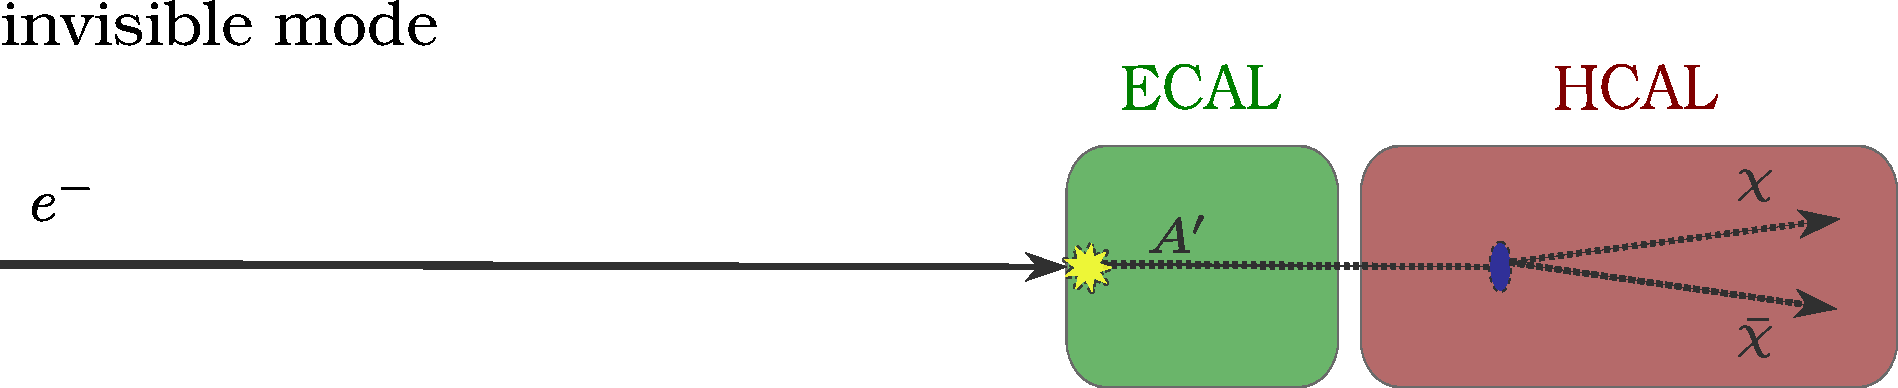
\includegraphics[width=\textwidth]{\pdirtwo/experiments-concepts-invisible.pdf}
  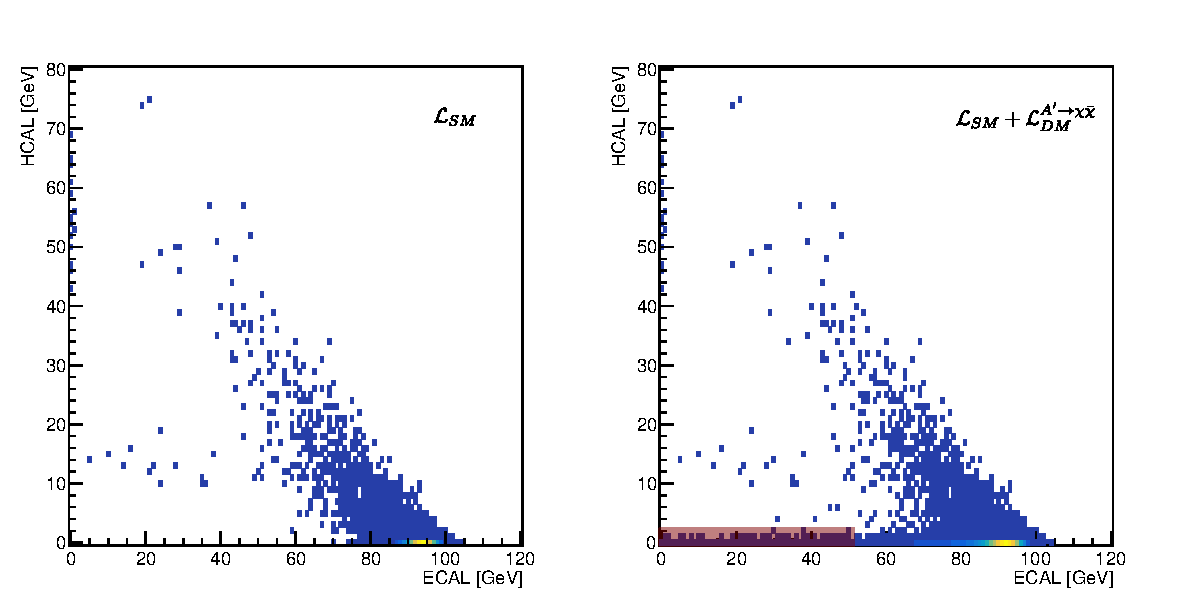
\includegraphics[width=\textwidth]{\pdirtwo/invisiblemode_signalregion.pdf} \\
  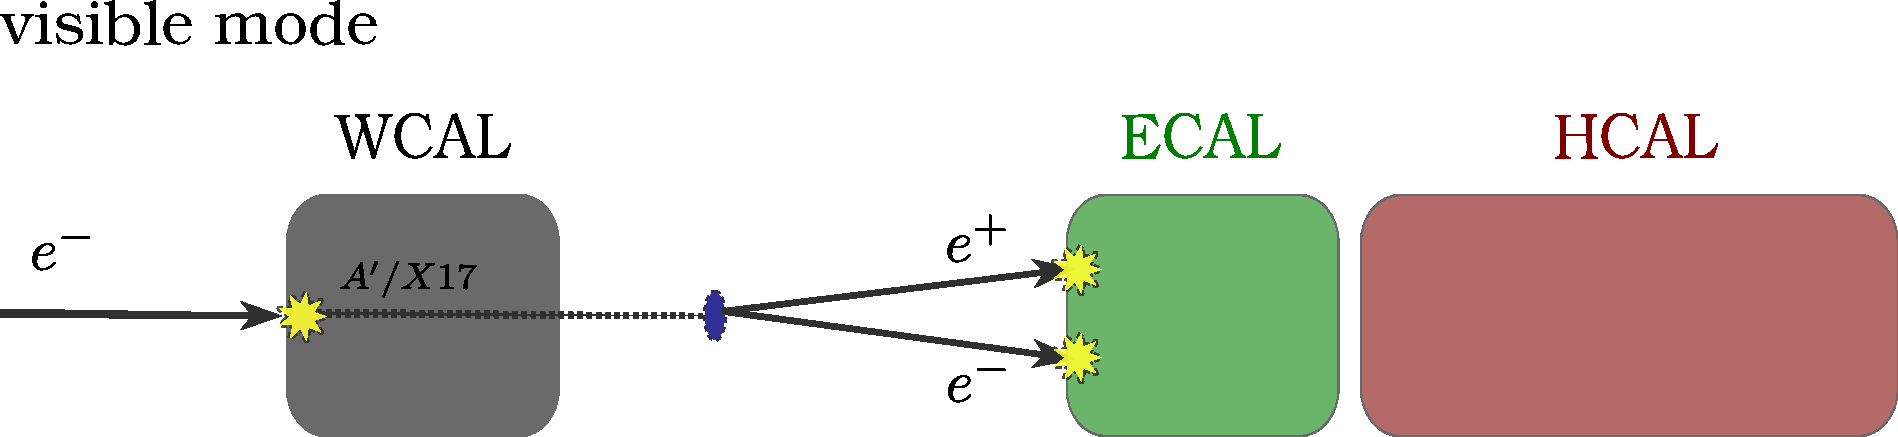
\includegraphics[width=\textwidth]{\pdirtwo/experiments-concepts-visible.pdf}
  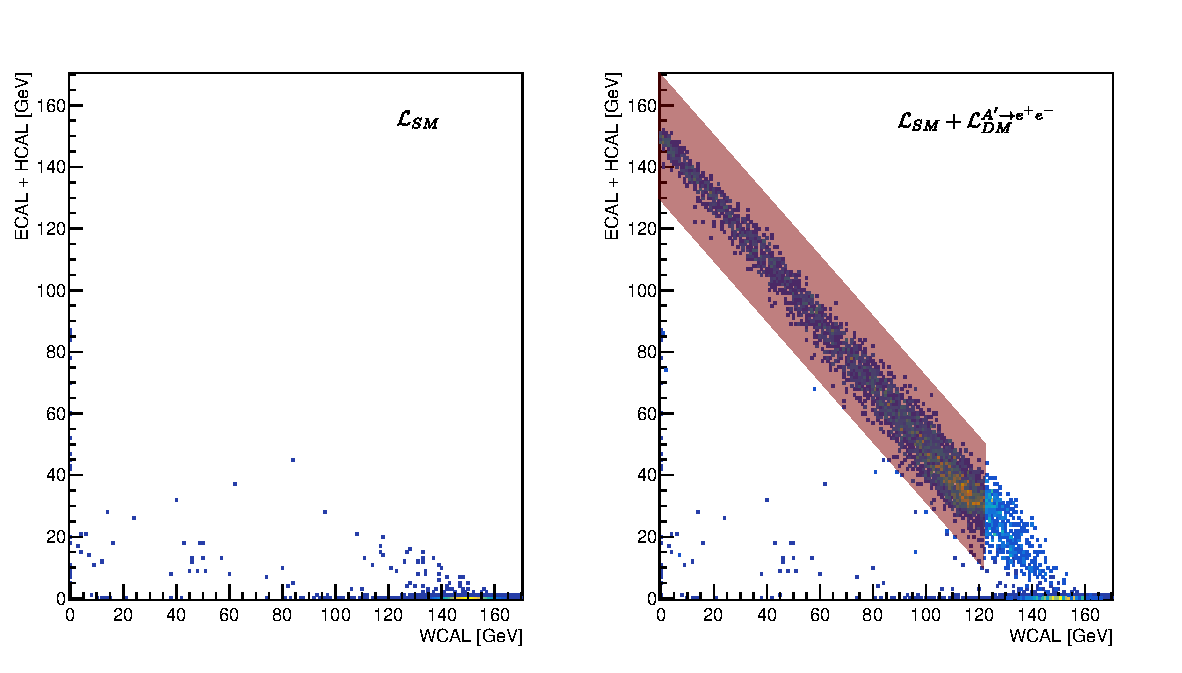
\includegraphics[width=\textwidth]{\pdirtwo/visiblemode_signalregion.pdf}   
\caption[Sketch of experimental signatures for $\DM$]{Sketch of the two possible signature in the NA64 setup to probe the $\DM$ existence. A heatmap present the event distribution in the two setups, using only standard model physics (left column) and after adding the Dark Photon production in the simulation. This is done assuming invisible mode decay $\ainv$ (top) or visible mode decay $\aee$ (bottom). In both cases, the signal region of the experiment is drawn as a shaded area.}
\label{fig:two-signature}
\end{figure}

\clearpage
\newpage

\section{Experimental setup}
\label{ch2:sec:experimental-setup}

The NA64 experiment uses the upgraded H4 electron beamline at CERN SPS. The beam is produced by the primary proton beam of 450 \si{\giga\electronvolt} with an intensity up to 5-7$\times$10$^{12}$ Proton On Target (POT) per SPS spill. The electrons are produced on a primary beryllium target and transported to the detector inside the evacuated beamline tuned to an adjustable beam momentum. A precise description of the beam apparatus is available in \cite{sps-beamline,h4-beamline}. The beam properties can be tuned with the magnetic field settings and other parameters. In the case of NA64, two different beam settings are used depending on which $\DM$ decay channel is being probed. In the case of the invisible decay $\ainv$, the beam momentum is tuned to 100 $\gev$. In this condition, a purity $\pi^-/e^- \lesssim 10^{-2}$ is achieved with a beam size of $\sim$1.5\si{cm} (FWHM). In the case of the visible decay $\aee$ on the other hand, a larger initial energy is used to boost the decay time of the $\DM$ and increase its chances of traveling outside the target. This is especially true for the $\DMX$, since an important portion of the parameter space justifying this anomaly is characterized by large couplings $\epsilon \gtrsim 10^{-3}$ and hence a very short decay time $\tau \lesssim 10^{-13}$\si{s}. In this case, the beam is tuned to 150 $\gev$ as a compromise between high-energy and acceptable reduction of the flux.

In the next sections, both setups used by NA64 will be described in detail. We will follow here a historical approach where the invisible mode setup is described first, as it was originally the first setup used in the test beam of 2016. In Sec.\ref{ch2:sec:vismode}, on the other hand, we will focus on the most important difference between this first setup and the one used to probe the visible mode.


\subsection{The invisible mode setup}
\label{ch2:sec:invismode}

The invisible mode setup used for data-taking in 2018 is presented in Fig.\ref{fig:setup-invis-2018}. After the e$^-$ primary enters the setup, its momentum is measured precisely to provide an initial estimate of its energy. This is achieved using a magnetic spectrometer with an integrated field of $\sim 7$ \si{\tesla\meter} generated by two dipole magnets \cite{mbpl} placed in series along the primary beam-axis. The entrance angle of the particle inside the magnet is defined by two Micromegas (MM) trackers placed inside the 5 m space between the beam inlet and the first magnet entrance. Between the two MM, in a space of approximately 2 m, two scintillators ($S_{0-1}$) and a $V$ counter ensure a proper beam definition. The $V$ counter consists of a scintillator with a hole in the middle and is used to reject particle with a high beam divergence that could in principle be a source of background. The two magnets are followed by a \SI{10.2}{\meter} long vacuum tube kept at 10$^{-3}$ \si{mbar} is placed immediately after with a total length of 10.2 \si{m}. The vacuum minimizes the interaction of the particles during their travel to the target. This is important to suppress the emission of secondary particles before the primary hits the target. As will be detailed in Sec.\ref{ch3:sec:bkg-srd}, the electron identification achievable with synchrotron radiation is also improved. After the vacuum tube, a space of $\sim$ \SI{4.5}{\meter} contains the last detectors before the target. A second set of three scintillators ($S_{2-3-4}$) completes the trigger system. Three sets of Pb-Sc sandwiches are placed in the arch contained between the original beam and the bent beam direction to collect the synchrotron radiation emitted in the magnetic field upstream. On the other side of the beam (see Fig.\ref{fig:setup-invis-2018}), a similar detector with no transversal segmentation (W sandwich) rejects events with high beam divergence or events in which the electron experienced a high-energy scattering upstream. Four more MM (MM$_{3-4-5-6}$) are located along the beam to complete the momentum reconstruction by detecting the displacement of the electron after its passage through the magnetic field. Eight more tracking detectors are placed before the ECAL: 2 Strawtubes (St), and 4 four Gas Electron Multiplier (GEM). The GEM detectors have a hit resolution and efficiency similar to the MM.
%, with the advantage of not being multiplexed, hence they experience less redundancy in the hit position. As it will be detailed in Sec.\ref{ch2:sec:detectors-tracking}, the multiplexing does not limit the momentum resolution and hence the final performance given are comparable overall.
The Strawtubes, on the other hand, posses a larger active area ($\sim$0.5 m), but a hit resolution of $\sim$1 $\mmi$ which makes them less suitable to reconstruct the momentum precisely \cite{Volkov:2019qhb}. This detector has however the virtue of being large enough to detect charged particle emitted at a large angle. Hence, it can reject rare events where the production by inelastic scattering of hadrons emitted at large angles causes some momentum to escape the setup transversely. These events are not rejected by the W alone and they can be a source of background for the large number of EOT required by the experiment \cite{na64-prd}. 

After this region, the primary electron hits the active target (ECAL). The ECAL is made of 36 modules arranged in a 6$\times$6 matrix, each module has a Pb-Sc structure with 150 layers for a total of 40$X_0$. Due to its transverse segmentation, the ECAL allows further background rejection using a shower profile analysis to distinguish between an em-shower and hadronic one. To ensure complete hermeticity, a high-efficiency VETO and a large Hadronic Calorimeter (HCAL) are placed after the ECAL target. The VETO consists of three separate scintillators stacked together resulting in a thickness of \SI{5}{\centi\meter}. Its rejection efficiency of Minimum Ionizing Particles (MIP) was estimated to be 99.9$\pm$0.1\%. The HCAL, located immediately after, consists of four modules of $\simeq$7 $\lambda_{int}$ (nuclear interaction length) each. Each module is built in a 3$\times$3 matrix of a single Fe-Sc sandwich array. The role of this last calorimeter is to block all possible particles penetrating the ECAL to grant complete energy hermeticity. In the past version of the setup, all four modules were stacked in series after the ECAL for a total of $\simeq$28 $\lambda_{int}$ \cite{Banerjee:2016tad}. In the last version of the setup, the last module is shifted to face the original beam axis (Fig.\ref{fig:setup-invis-2018}). This allow to detect large bremsstrahlung photons emitted before the magnet by the incoming electrons. A more detailed description of the NA64 detectors can be found in \ref{ch2:sec:detectors}.

\begin{figure}[tbh!]
  \centering
  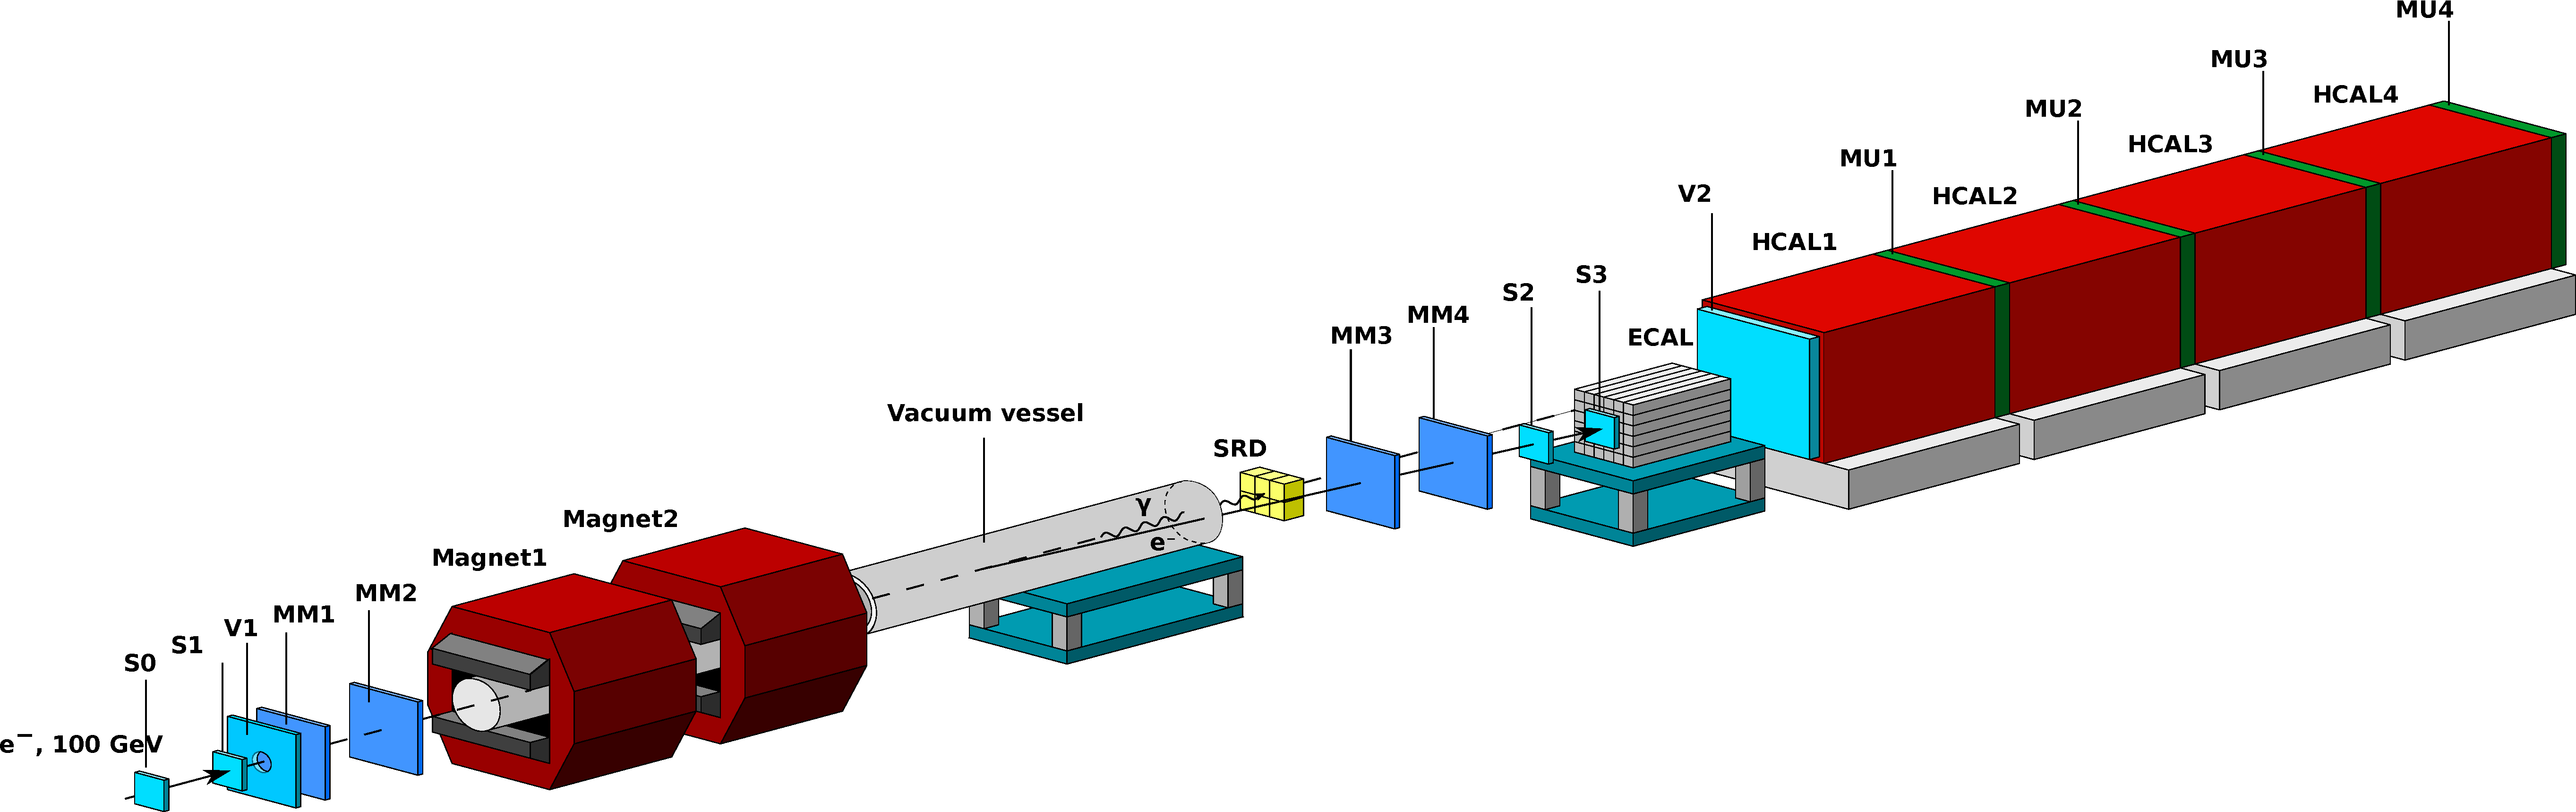
\includegraphics[width=\textwidth]{\pdirtwo/invisible_mode_setup.pdf}
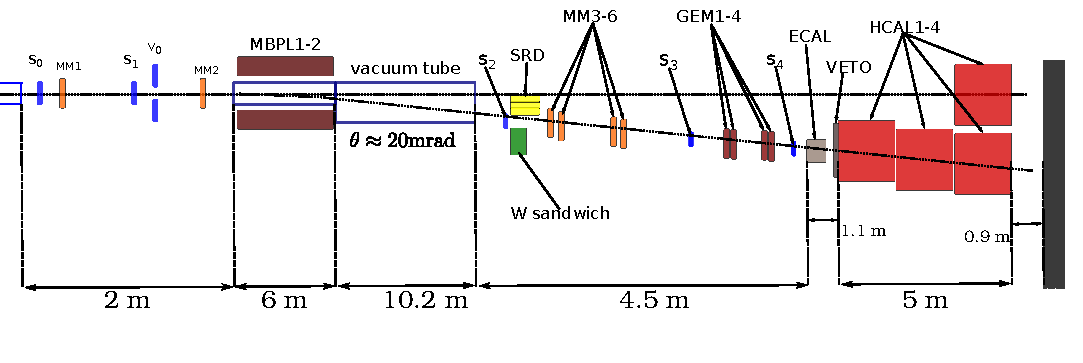
\includegraphics[width=\textwidth]{\pdirtwo/setup-invis-2018.pdf}
\caption[invisible mode setup 2018]{Top: Invisible mode setup sketched in 3D. Main detectors are shown. Dummy decay of a $\DMX$ after the dump is depicted. Bottom: Top view of the invisible mode setup used in 2018, all detectors included.}
\label{fig:setup-invis-2018}
\end{figure}

\subsection{The visible mode setup}
\label{ch2:sec:vismode}

The visible mode setup is obtained by modifying slightly the invisible mode setup to accommodate a long decay volume where the $\ee$ pair from the $\DM$ decay would be measured by a scintillator counter and four GEM stations (Fig.\ref{fig:setup-vis-2018}). The energy of the beam is increased to 150 GeV\footnote{First run in 2017 was performed at 100 $\gev$.}. The reason for this is to boost the $\DM$ decays outside the dump. As a consequence, the total displacement of the primary beam caused by deflection in the magnetic field is roughly $\sim$\SI{10}{\milli\meter} smaller. Since the space between the origin and bent beam axis is reduced, only two modules of the SRD detector fit in this space, which decreases the suppression of heavy charged particles. Additionally, the smaller bending has an impact on the momentum reconstruction as well, less significant for this analysis. A compact calorimeter made of a Tungsten-scintillator sandwich (WCAL) is planted in front of the ECAL and acts as the target in this new setup. This calorimeter has a total of 30$X_0$ in a compact length of $\sim$20 \si{cm}. The $\DM$ is produced via scattering off nuclei in this active dump, followed by its decay $\aee$ after traveling for some distance without interaction. To ensure that the decay happens after the dump, the last layer of the WCAL is read separately (W2). This also acts as a veto to reject high energetic particles that leak from the em-shower. A vacuum tube of 3.1 \si{m} kept at $\sim$10$^{-2}$ \si{mbar} is used to minimize interactions of the $\ee$. A scintillator (S$_4$), is placed immediately after the tube to detect the presence of the $\ee$ pair with a double-MIP signal inside this counter. A set of four GEM detectors are then placed in the last $\simeq$2.5 \si{m} of air before the second active target (ECAL). In principle, these four trackers can reconstruct the angle and the vertex of the decay to offer an additional characterization of the signal. These tools were not used in the analysis performed in 2018 \cite{Banerjee:2019hmi}, but in this thesis, an analysis considering the trackers as well is described (see Sec.\ref{ch3:sec:vis-mode-tracking}). Finally, the ECAL detects the remaining energy of the two $\ee$ pair in the decay volume, and matches it to the one measured in the WCAL. If the sum $E_{WCAL}+E_{ECAL}$ is compatible with the initial primary energy E$_0$, we conclude that some energy escaped the WCAL using new physics. At the end of the setup, a high-efficiency VETO and the HCAL are still present to guarantee complete hermeticity. One could question the usefulness of these detectors here, indeed if we can guarantee that only 150 GeV $e^-$ are in the system, the simple requirement of energy conservation should be enough to reject all backgrounds coming from impurities in the beam. The limited energy resolution of the two calorimeters, however, can produce a wrong measurement that implies energy conservation. Likewise, a pileup event of two particles in the same trigger can produce the same effect. On top of this, the HCAL is used to properly estimate the hadron contamination of the beam and to select rare events containing the interaction $\emu$ where two muons are produced in the dump inside the em-shower. As we will see this type of event is crucial for our analysis to properly account for the systematic of the experiment, both in the invisible and visible mode, which makes the HCAL and VETO necessary in both setups.

\begin{figure}[tb]
  \centering
  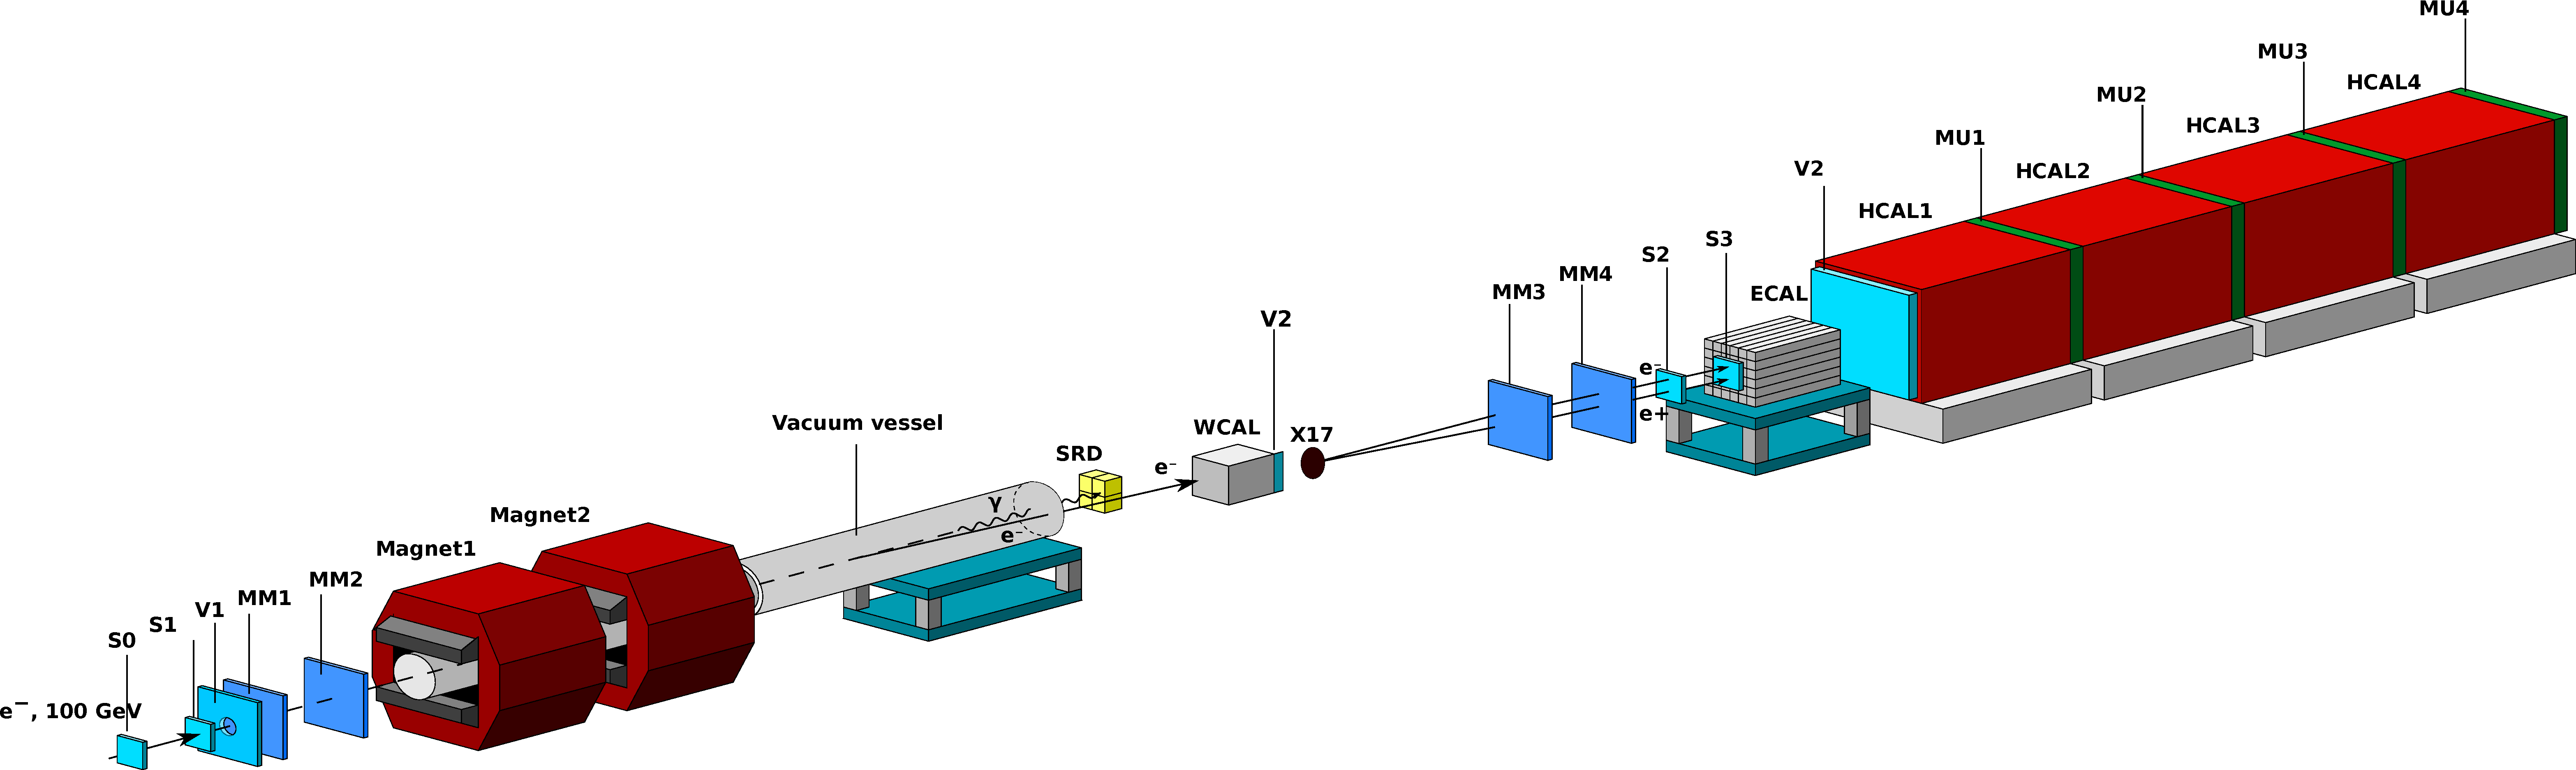
\includegraphics[width=\textwidth]{\pdirtwo/visible_mode_setup.pdf}  
  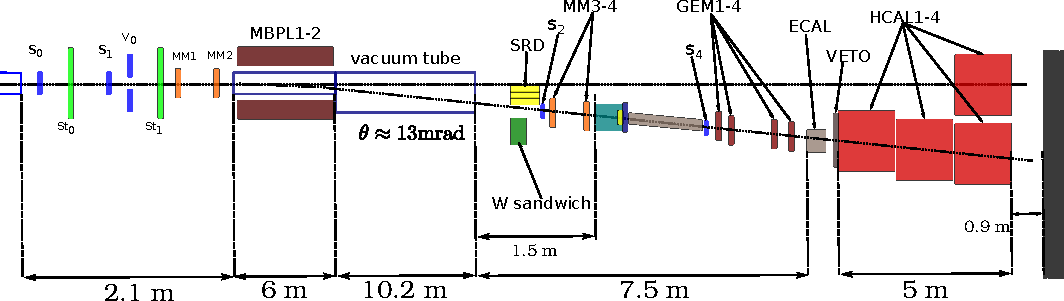
\includegraphics[width=1.\textwidth]{\pdirtwo/NA64_setup_2018_visible.pdf}
  \caption[NA64 visible mode setup 2018]{Top: Visible mode setup sketched in 3D. Main detectors are shown. Bottom: Top view of the visible mode setup used in 2018, all detectors included.}
  \label{fig:setup-vis-2018}
\end{figure}

\section{Detectors}
\label{ch2:sec:detectors}

In this section, the various detectors that are used to build the two setups are described in more detail to give a technical overview of each component. More information about each detector can be found in \cite{na64-hcal,na64-detectors,ABBON201569}. A summary table with all technical details is also provided in Table \ref{tab:detector-tables}.

\subsection{The Trigger system}
\label{ch2:sec:detectors-trigger}

The trigger system is based on the coincidence and anti-coincidence of different scintillator counters placed along the beam directions combined with the requirement of specific energy in the primary active dump (the ECAL in the invisible mode and the WCAL in the visible mode).

Five plastic scintillators (S$_{0-4}$) and one Veto (V) are used for this purpose. They have a variable diameter ranging from 32 to 42 \si{mm} and a thickness of 3-5 \si{mm}. The sandwich S$_0$-V-S$_1$ is placed in front of the beam inlet to characterize the initial particle direction. To pass this first step of the trigger, a particle needs to leave a signal of at least 0.8 $\emip$ in S$_{0-1}$ and no signal in V. Where $\emip$ is the Most Probable Value (MPV) of energy deposited by a MIP inside the active volume\footnote{The distribution of energy deposited by a MIP inside a material is a Landau distribution, where the MPV is one of the fundamental parameters defined by the thickness and the density of the material crossed by the particle.}. This is expressed by the condition:

\begin{equation}
\label{eq:trigger-upstream}
Tr_U = S_0 \cdot \bar{V} \cdot S_1
\end{equation}

The signal needs to be in a coincidence compatible with the time resolution of the two scintillators ($\simeq$3 \si{ns}) to suppress the pileup. Downstream, three more scintillators are placed (S$_{2-4}$) in the case of the invisible mode and a coincidence of all three is also required as a part of the trigger downstream. In the case of the visible mode, only the first of three scintillators (S$_2$) is part of the trigger, S$_3$ is removed and S$_4$ is placed after the decay for analysis purpose without being a direct part of the trigger. This means:

\begin{equation}
\label{eq:trigger-downstream}
\begin{split}      
& Tr^{invis}_D = S_2 \cdot S_3 \cdot S_4 \\
& Tr^{vis}_D = S_2 \\
& Tr^{invis/vis}_{U+D} = Tr_U \cdot Tr^{invis/vis}_D
\end{split}
\end{equation}

We notice that the scintillator counters downstream are small enough to already limit significantly the range of momenta accepted in the trigger of the experiment ($\gtrsim$ 90 $\gev$)). However, large beam divergences coupled to pileup can still potentially cause a low energy $e^-$ inside the trigger window, hence the
necessity of a tracking system. As a final tool for the beam definition, a small energy deposit in W is required, to reject events with large upstream bremsstrahlung. The exact threshold depends on the exact run, but it is always in the range of 3-6 $\gev$. We define the beam-trigger as the sum of all these components in the two different setups:

\begin{equation}
\label{eq:trigger-beam}
Tr_{beam} = Tr_{U+D} \cdot \bar{W}
\end{equation}

Finally, as the DAQ can collect data at a rate of $\simeq$10 \si{kHz}, one needs an additional condition to select only those events that have a chance to be in the signal region. In both setups, this means some missing energy in the primary target-dump. Additionally, since both WCAL and ECAL have some longitudinal segmentation, one can use the pre-shower information to suppress the hadron background at the trigger level. This is achieved by splitting the signal in these modules to feed them to a discriminator. The trigger, in this case, has the following form:

\begin{equation}
\label{eq:trigger-phys}
\begin{split}
& Tr^{invis}_{phys} = ECAL^{presh}(> \SI{300}{\mega\electronvolt}) \cdot ECAL(<\SI{85}{\giga\electronvolt})\\
& Tr^{vis}_{phys} = WCAL^{presh}(>\SI{500}{\mega\electronvolt}) \cdot WCAL(<\SI{110}{\giga\electronvolt})
\end{split}
\end{equation}

The final trigger during data taking will be a combination of both the primary trigger for the beam definition and the physical trigger used to obtained a rate that can be handled by the DAQ. We obtain finally:

\begin{equation}
\label{eq:trigger-total}
\begin{split}
& Tr^{invis}_{total} = S_0 \cdot \bar{V} \cdot S_1 \cdot S_2 \cdot S_3 \cdot S_4 \cdot \bar{W} \cdot ECAL^{presh}(> \SI{300}{\mega\electronvolt}) \cdot ECAL(<\SI{85}{\giga\electronvolt})\\
& Tr^{vis}_{total} = S_0 \cdot \bar{V} \cdot S_1 \cdot S_2\cdot \bar{W} \cdot WCAL^{presh}(>\SI{500}{\mega\electronvolt}) \cdot WCAL(<\SI{110}{\giga\electronvolt})
\end{split}
\end{equation}

The precise definition of the trigger varies between different runs. In general, we can define three different categories:

\begin{itemize}
\item \textbf{Hadron calibration run:} Where $\pi^-$ are used as primary particle and only $Tr_{beam}$ is used. These runs are used to measure precisely the interaction of hadrons in the setup and to study the background suppression in NA64. Their intensity is suppressed due to the thick target placed inside the beamline ($\approx 10^{3}$ $\pi^-$\si{\per\second}).
\item \textbf{Electron calibration run:} Where $e^-$ is used as primary particle and only $Tr_{beam}$ is used. These runs are used to measure the typical interaction of an EOT without a physical trigger. 
\item \textbf{Physical run:} Where $e^-$ is used as primary particle and $Tr_{total}$ is used. These runs are used to collect the data for the analysis. 
\end{itemize}

Although the Physical runs use an electron beam, the physical trigger naturally selects events with hadrons as a primary particle. The vast majority of $e^-$ will deposit all their energy inside the target-dump, and are thus rejected by the physical trigger. This means that the sample of events recorded will have a large percentage of hadrons that will be rejected by the selection criteria. To properly account for the cuts efficiency, electron and hadron calibration runs are used, since the impurity of the sample is known and easy to remove.

\subsection{The Electromagnetic Calorimeter (ECAL)}
\label{ch2:sec:detectors-ecal}

The electromagnetic calorimeter shown in Fig.\ref{fig:ecal-sketch} is a shashlik type detector design for energy measurement, shower profile measurement, and $e/\pi$ separation. Its design consist in a 6$\times$6 matrix of single modules with dimension 38.2$\times$38.2$\times$471 $\mmc$. Each cell consists of 150 layers, which in turn are made of 1.5 $\mmi$ as converter layer, 0.14 $\mmi$ of paper as the separator, and 1.5 $\mmi$ for energy measurement. This is equivalent to 40$X_0$ radiation length. The single cell is further divided into two different longitudinal segments. The first one is called pre-shower and consists of 16 layers ($\sim$4.27$X_0$) and gives resolution to the very beginning of the shower. Since $e^-$ and $\gamma$ trigger an em-shower very early (with the $\gamma$ being a bit delayed within respect to the electron. see \cite{Bichsel:2002cf}), this information can be used to discriminate such particles from all the ones with higher penetrating power (mostly $\pi^-$ and $\mu^-$ in the NA64 case). The second part called simply main ECAL consist of 134 layers ($\sim$35.73$X_0$), and its purpose is to completely stop the incoming particle to measure its energy. The light collection of the scintillator part is performed by Wave Length Shifter (WLS) fibers BCF91a \cite{wls-fibers} inserted in a spiral along with the cell to avoid energy leak through them. The Calorimeter is calibrated using a low-intensity electron beam where a mechanical support structure is used to move every single cell on the beam center. The pre-shower and the main calorimeter are then calibrated using a Gaussian fit and the precise energy fraction between the two longitudinal segments is calculated through a detailed MC simulation. The energy resolution estimated for this detector is of $10\% / \sqrt{E[\gev]}$.

\begin{figure}[bth!]
\centering
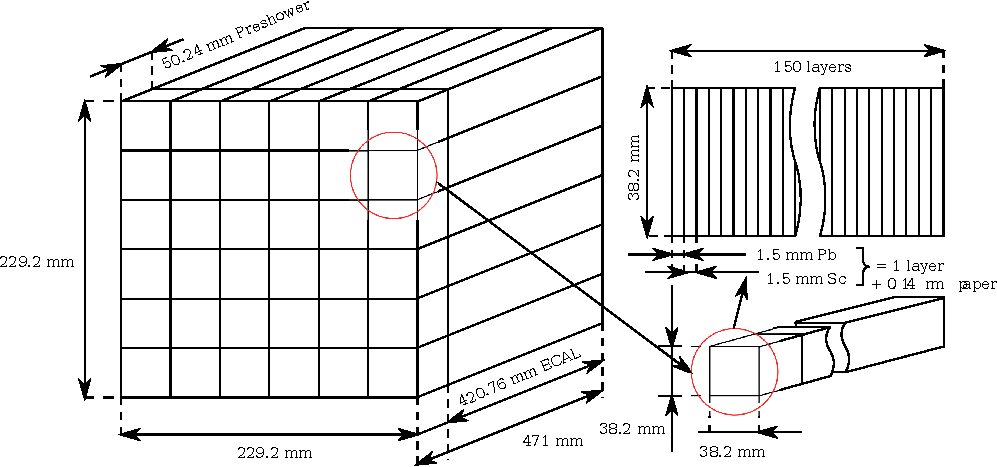
\includegraphics[width=\textwidth]{\pdirtwo/ECAL.pdf}
\caption[ECAL sketch]{Technical sketch of the Shaslik type calorimeter.}
\label{fig:ecal-sketch}
\end{figure}

\subsection{The Electromagnetic Tungsten Calorimeter (WCAL)}

The Tungsten electromagnetic calorimeter (Fig.\ref{fig:wcal-sketch}) is another shashlik type detector design to stop high-energy particles in a short length. Its structure consists of a sandwich of Tungsten and scintillator counters for a total of 35 layers. Each layer consists of 3 $\mmi$ of Tungsten and 2 $\mmi$ of scintillator material, for a total radiation length of $\sim$30$X_0$. Its dimension is 150$\times$150$\times$200 $\mmc$, including the Aluminum box used to hold the detector together. The total transverse size of the active area is 120$\times$120 $\mms$. The readout uses the same WLS fiber used for the ECAL readout by PMTs, for a total energy resolution achieved of $20\%/ \sqrt{E[\gev]}$. The WCAL is not transversely segmented as the ECAL but is segmented longitudinally in three different sections. The first one, called pre-shower, consist of the first 5 layers of the calorimeter, which are used to increase the $e/\pi$ separation. The second one is the main calorimeter, made of the remaining 30 layers, and acts as the main active target to stop the incoming $e^-$ completely and measure their energy. The last part is the veto, called W2, which consist of three scintillator counters stacked in series and read out by a single PMT, for a total active dimension of 60$\times$120 $\mms$. The purpose of this last detector is to measure the leaking of the em-shower from this calorimeter to reject events with leaking charged particles. The calorimeter is used in the visible mode as an active target, and its design allows the setup to be sensitive to particles with short decay length.

\begin{figure}[bth!]
\centering
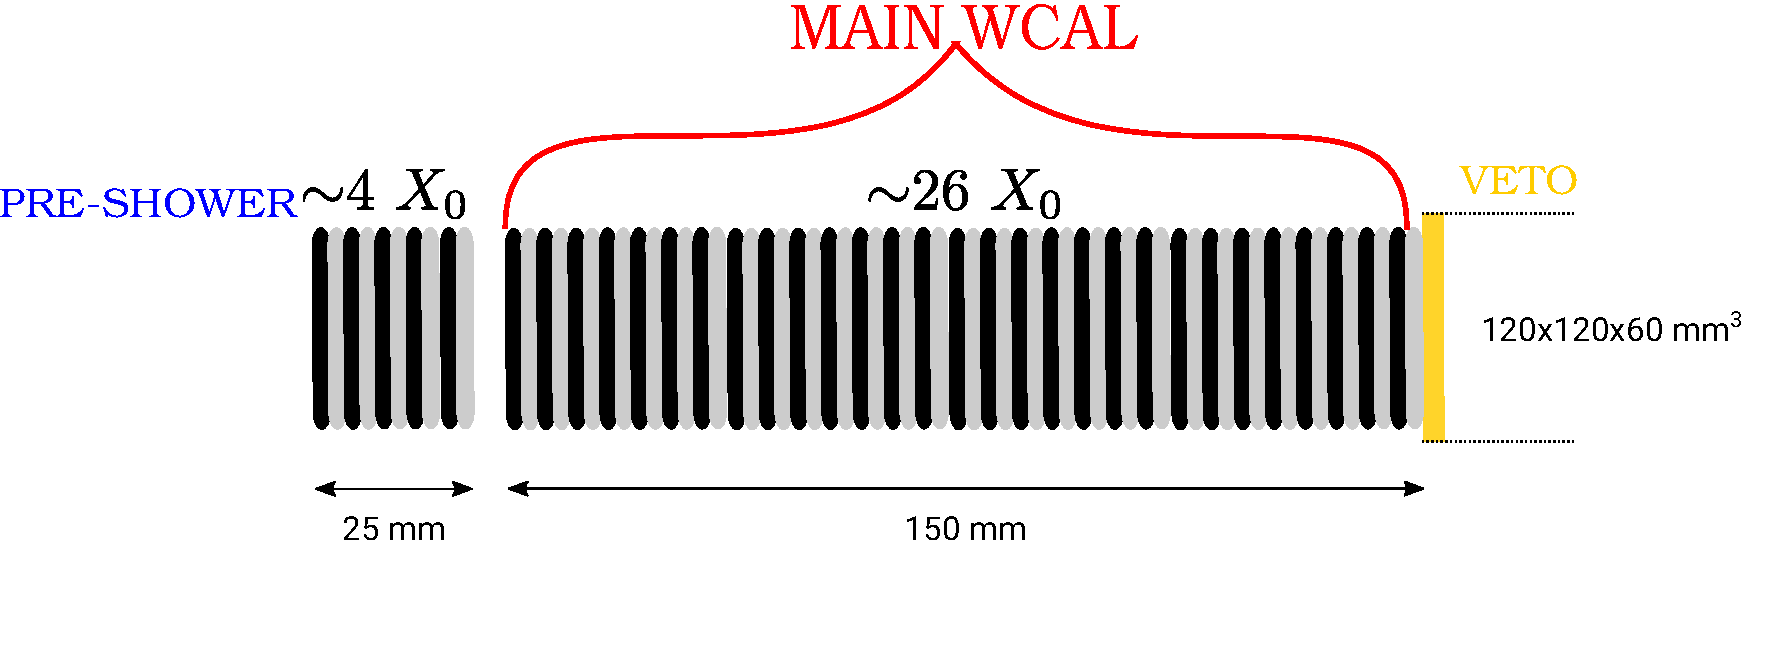
\includegraphics[width=\textwidth]{\pdirtwo/WCAL.pdf}
\caption[WCAL sketch]{Technical sketch of the WCAL module used in the NA64 experiment.}
\label{fig:wcal-sketch}
\end{figure}


\subsection{The Hadronic Calorimeter (HCAL)}
\label{ch2:sec:detectors-hcal}

The hadronic calorimeter in the NA64 experiment consists of four modules and its primary purpose is to stop and reconstruct the energy of a high penetrating particle. This includes the $\pi^-$ and $K^-$ contained as impurities in the beam but also neutrons and protons that can be produced in inelastic scattering in the ECAL. Additionally, although a complete stop of 100 GeV $\mu^-$ remains unfeasible, the HCAL can characterize very efficiently the presence of such particle after the ECAL. The $\mu^-$ will leave the very distinctive $\emip$ energy deposit inside each module, amounting roughly to $\sim 2.5$ $\gev$. Each module of the HCAL is a 3$\times$3 matrix of cells. Each cell is a sandwich of alternating layers of 25 $\mmi$ Iron (Fe) and 4 $\mmi$ of scintillating material separated by a 9 $\mmi$ gap of air. Each cell consists of 48 layers for a total thickness of $\simeq 7\lambda_{int}$. The lateral size of each module is 194$\times$192 $\mms$. The light readout is analogous to the one of the ECAL, using WLS-fibers embedded in round grooves in the scintillator plates. The fibers from each cell are collected together in a single optical connector at the side of the module. Each of the 9 optical connectors is then read-out by a single photomultiplier. Similar to the ECAL, these modules are calibrated using special runs where 50 $\gev$ $\pi^-$ are shoot at different cells with the help of a mechanical table. The energy resolution estimated for this detector is $\sim 50\%/\sqrt{E[GeV]}$

\begin{figure}[bth!]
\centering
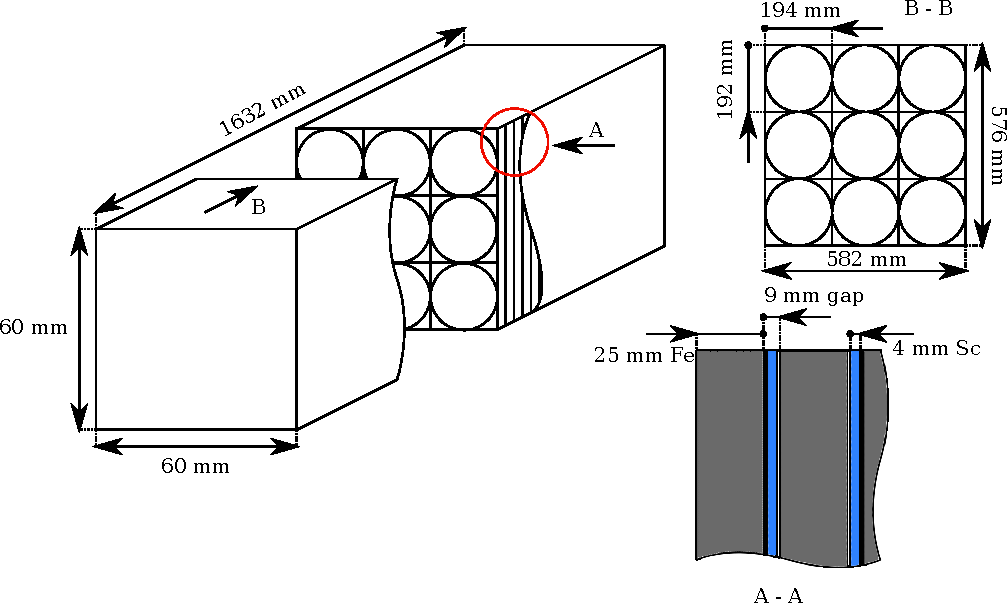
\includegraphics[width=\textwidth]{\pdirtwo/HCAL.pdf}
\caption[HCAL sketch]{Technical sketch of the HCAL module used in the NA64 experiment.}
\label{fig:hcal-sketch}
\end{figure}

\subsection{The Synchrotron radiation detector (SRD)}
\label{ch2:sec:detectors-srd}

The Synchrotron radiation detector (SRD) is a calorimeter placed downstream in the arc described by the original beam axis and the bent beam. Its purpose is to measure the energy of the photon emitted by the passage of each electron in the magnetic field downstream. The energy range of such a signal is in the order of a few tens of MeV, thus a larger precision is needed compared to the calorimeters used to measure the primary beam. Heavy charged particle suppression will be described more in detail in Sec.\ref{ch3:sec:bkg-srd}.

Historically, the first Synchrotron radiation detector used was a set of 8 BGO crystals arranged in 2$\times$4 matrices placed parallel to the beam direction. Each crystal has a hexagonal shape with a diameter of 61 $\mmi$ and a length of 200 $\mmi$. The light readout consists of an EMI PMT 9603 mount on the bottom of each crystal with optical grease. The BGO are excellent candidates for the SRD, due to the high light-yield and radiation length which coupled to their high Z makes them excellent gamma-absorbers \cite{bgo-crystal}. Indeed their rejection power can be as large as $10^{-4}$ and was demonstrated experimentally in the NA64 experiment (see Sec.\ref{ch3:sec:bkg-srd} for details). However, their large decay time of $\sim$300 \si{ns} creates a level of pileup that limits significantly their usefulness in a context where the intensity of the beam is very high.

The BGO detector was substituted with a shashlik type detector since the 2017 beam time, which uses three adjacent cells of dimension 60$\times$80 $\mmi$. Each cell consists of 100 layers with a lead-scintillator structure with dimensions 0.1 $\mmi$ and 1.1 $\mmi$ respectively. The light is read out by an R9420-100-10 Hamamatsu PMT with extended green spectral sensitivity \cite{hamamatsu-R9420-100-10}.

The time resolution for the shashlik type SRD is of $\sim$5 \si{ns}, which grants a suppressed pileup even at the largest intensity allowed in the H4 beamline.

\begin{figure}[bth!]
\centering
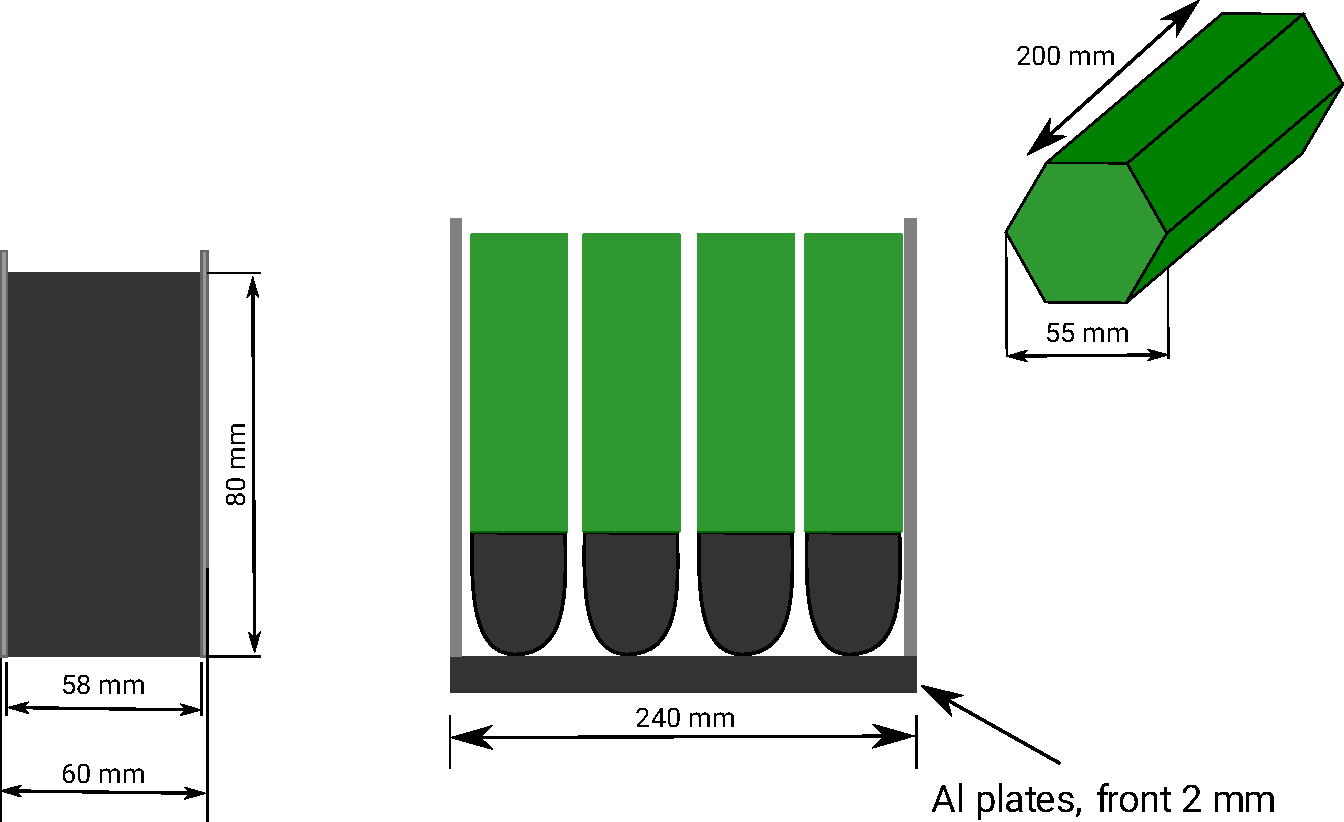
\includegraphics[width=\textwidth]{\pdirtwo/BGO.pdf}
\caption[BGO sketch]{Technical sketch of BGO crystal array.}
\label{fig:bgo-sketch}
\end{figure}

\begin{figure}[bth!]
\centering
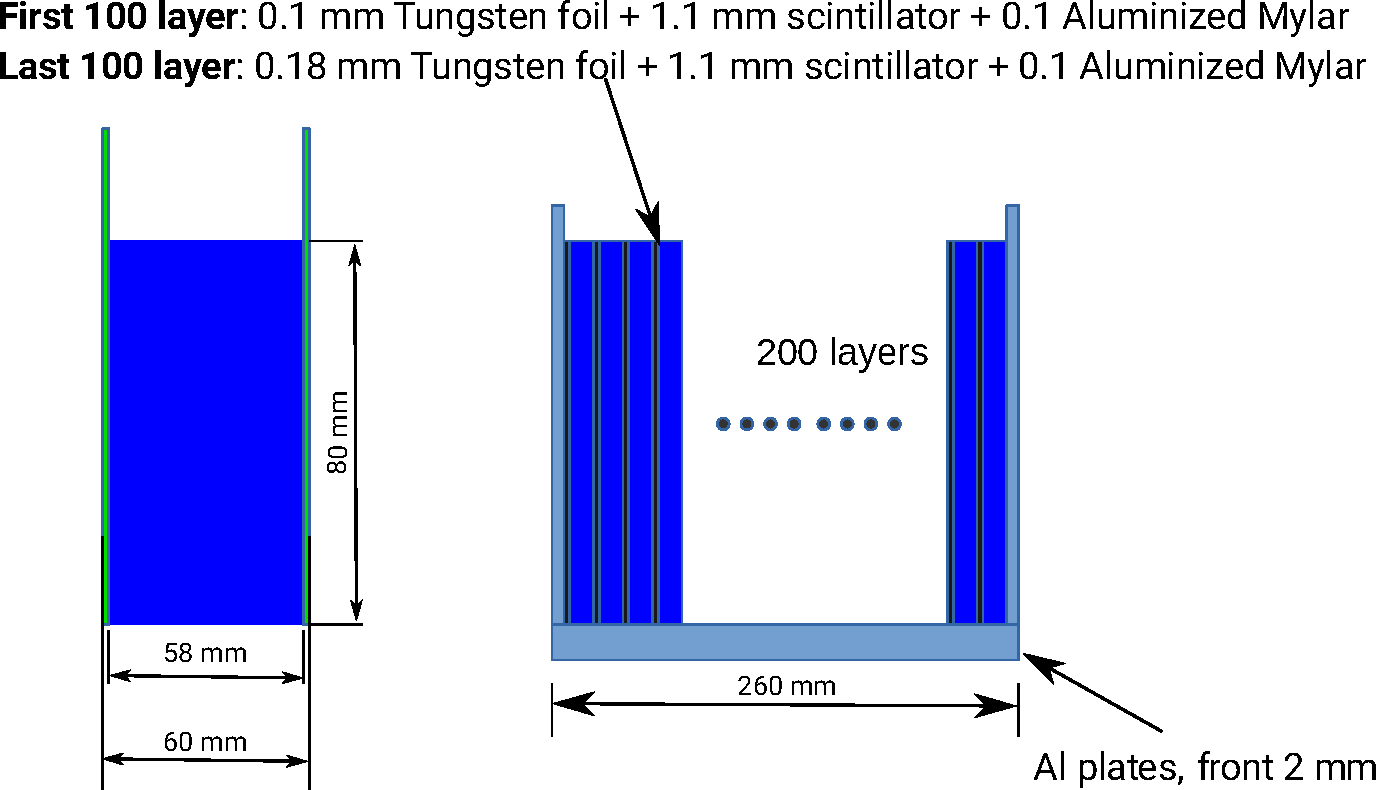
\includegraphics[width=\textwidth]{\pdirtwo/SRD.pdf}
\caption[SRD sketch]{Technical sketch of a single shashlik type module used in the NA64 experiment as SRD.}
\label{fig:srd-sketch}
\end{figure}

\subsection{The Veto system}
\label{ch2:sec:detectors-veto}

The Veto system is the set of thick scintillator counters with the purpose of measuring charged particles penetrating the main active target.

The most relevant detector of this type is the VETO, a set of three scintillators mounted in series for a total dimension of 550$\times$550$\times$50 $\mmc$. The MIP inefficiency of this detector is estimated to be $\sim 10^{-3}$.

For the visible mode, it is crucial to maintain the dump as short as possible to increase the probability of the $\aee$ decay to be outside of the dump. For this purpose, the last layers of the WCAL sandwich are decoupled from the main readout and used as a veto (called W2). The dimensions of this counter are hence connected to the one of the WCAL: 23$\times$23$\times$6 $\mmc$. For testing purposes, a second thicker counter (called V2) is still placed at a distance of $\sim3$ \si{cm} from W2 to cross-check its inefficiency.

In general, a signal event in both visible and invisible mode needs to be characterized by the absence of energy in the veto counter placed behind that target dump. In practice, events with an energy deposit $<$0.8 $\emip$ are accepted, taking into account both pedestal and energy resolution of these detectors.

\subsection{The Tracking system}
\label{ch2:sec:detectors-tracking}

The tracking system is the set of detectors that allows the full momentum reconstruction and track propagation in the NA64 setup. Four types of detectors are used to reconstruct hits position: Micromegas (MM), Gas Electron Multiplier (GEM), and Straw chambers (St$_i$). To this date only MM trackers are used as a direct part of the tracking system. In this thesis, however, a new analysis of the visible mode data is proposed that uses data from the GEM trackers to reconstruct the vertex position and the angles of the particles in the decay volume.

The exact working principle of each of these detectors is beyond the scope of this thesis. This section will be dedicated mostly to the description of the Micromegas detector, which was also one of my main responsibilities inside NA64. More information on the Straw chamber used in NA64 can be found in \cite{pdegen-thesis}.

\subsubsection{Micromegas}

Micromegas trackers are a set of eight Multiplexed XY Resistive Micromegas detectors (MM$_{1-8}$) used to reconstruct the 2D hit position of the incoming particles in the NA64 experiment. The design and original testing of the first modules were already the topics of a previous ETHZ thesis \cite{dbanerjee-thesis}. For completeness, in this section we will review its working principle and characteristic. As shown in Fig.\ref{fig:mm-sketch}, the primary particle enters the gas box where it ionizes some secondary electrons. In NA64, the gas is a mixture of Argon (93\%) and CO2(7\%). While Argon as noble gas is excellent to trigger the ionization, the C02 acts as a quencher to absorb UV-light emitted to avoid an excessive ionization that would both decrease the hit resolution and saturate the detector. The secondary electrons are then guided by the drift field in the amplification gap. The amplification gap is separated from the drift gap with a mesh formed by 400 wires with an aperture size of $\sim$45 $\mum$, wire diameter $\sim$18 $\mum$ and thickness of the mesh of $\sim$ 29 $\mum$. The secondary electrons reaching the amplification gap experience a high electric field of $\sim$ \SI{50}{\kilo\volt\per\centi\metre} which triggers a secondary avalanche that multiplies the electrical charge, collected in the strips of the PCB\footnote{Printed Circuit Board}. While the choice of the amplification field is typically set by the breakdown voltage of the gas, the choice of the drift voltage is not constrained, but a value too large can impact the transparency of the mesh effecting the efficiency of the detector. As pointed out in \cite{Bortfeldt:2014vvt}, an electric field of \SI{0.6}{\kilo\volt\per\centi\metre} is a good rule of thumb to maximize the efficiency. Another problem for MM comes from the thin amplification region that makes them particularly vulnerable to sparks, which happens when the total number of electrons in the avalanche reaches the value of a few $\sim 10^7$, called Raether limit \cite{BAY2002162,BRESSAN1999321,Raether:102989}. Additionally to the damage the detector and the readout electronics, a spark can also lead to a dead time and thus to a significant reduction of its efficiency. The introduction of resistive strips, which add a continuous RC circuit on the top of the readout strip plane, leads to the spreading of charge which avoids spark development and the voltage drop. These strips are grounded and separated from the readout strips via a thin insulating layer. The charge is therefore not directly collected by the cooper strips. Instead, an electrical signal is generated via capacitive coupling between the resistive and readout strips.

\begin{figure}[bth!]
  \centering
  %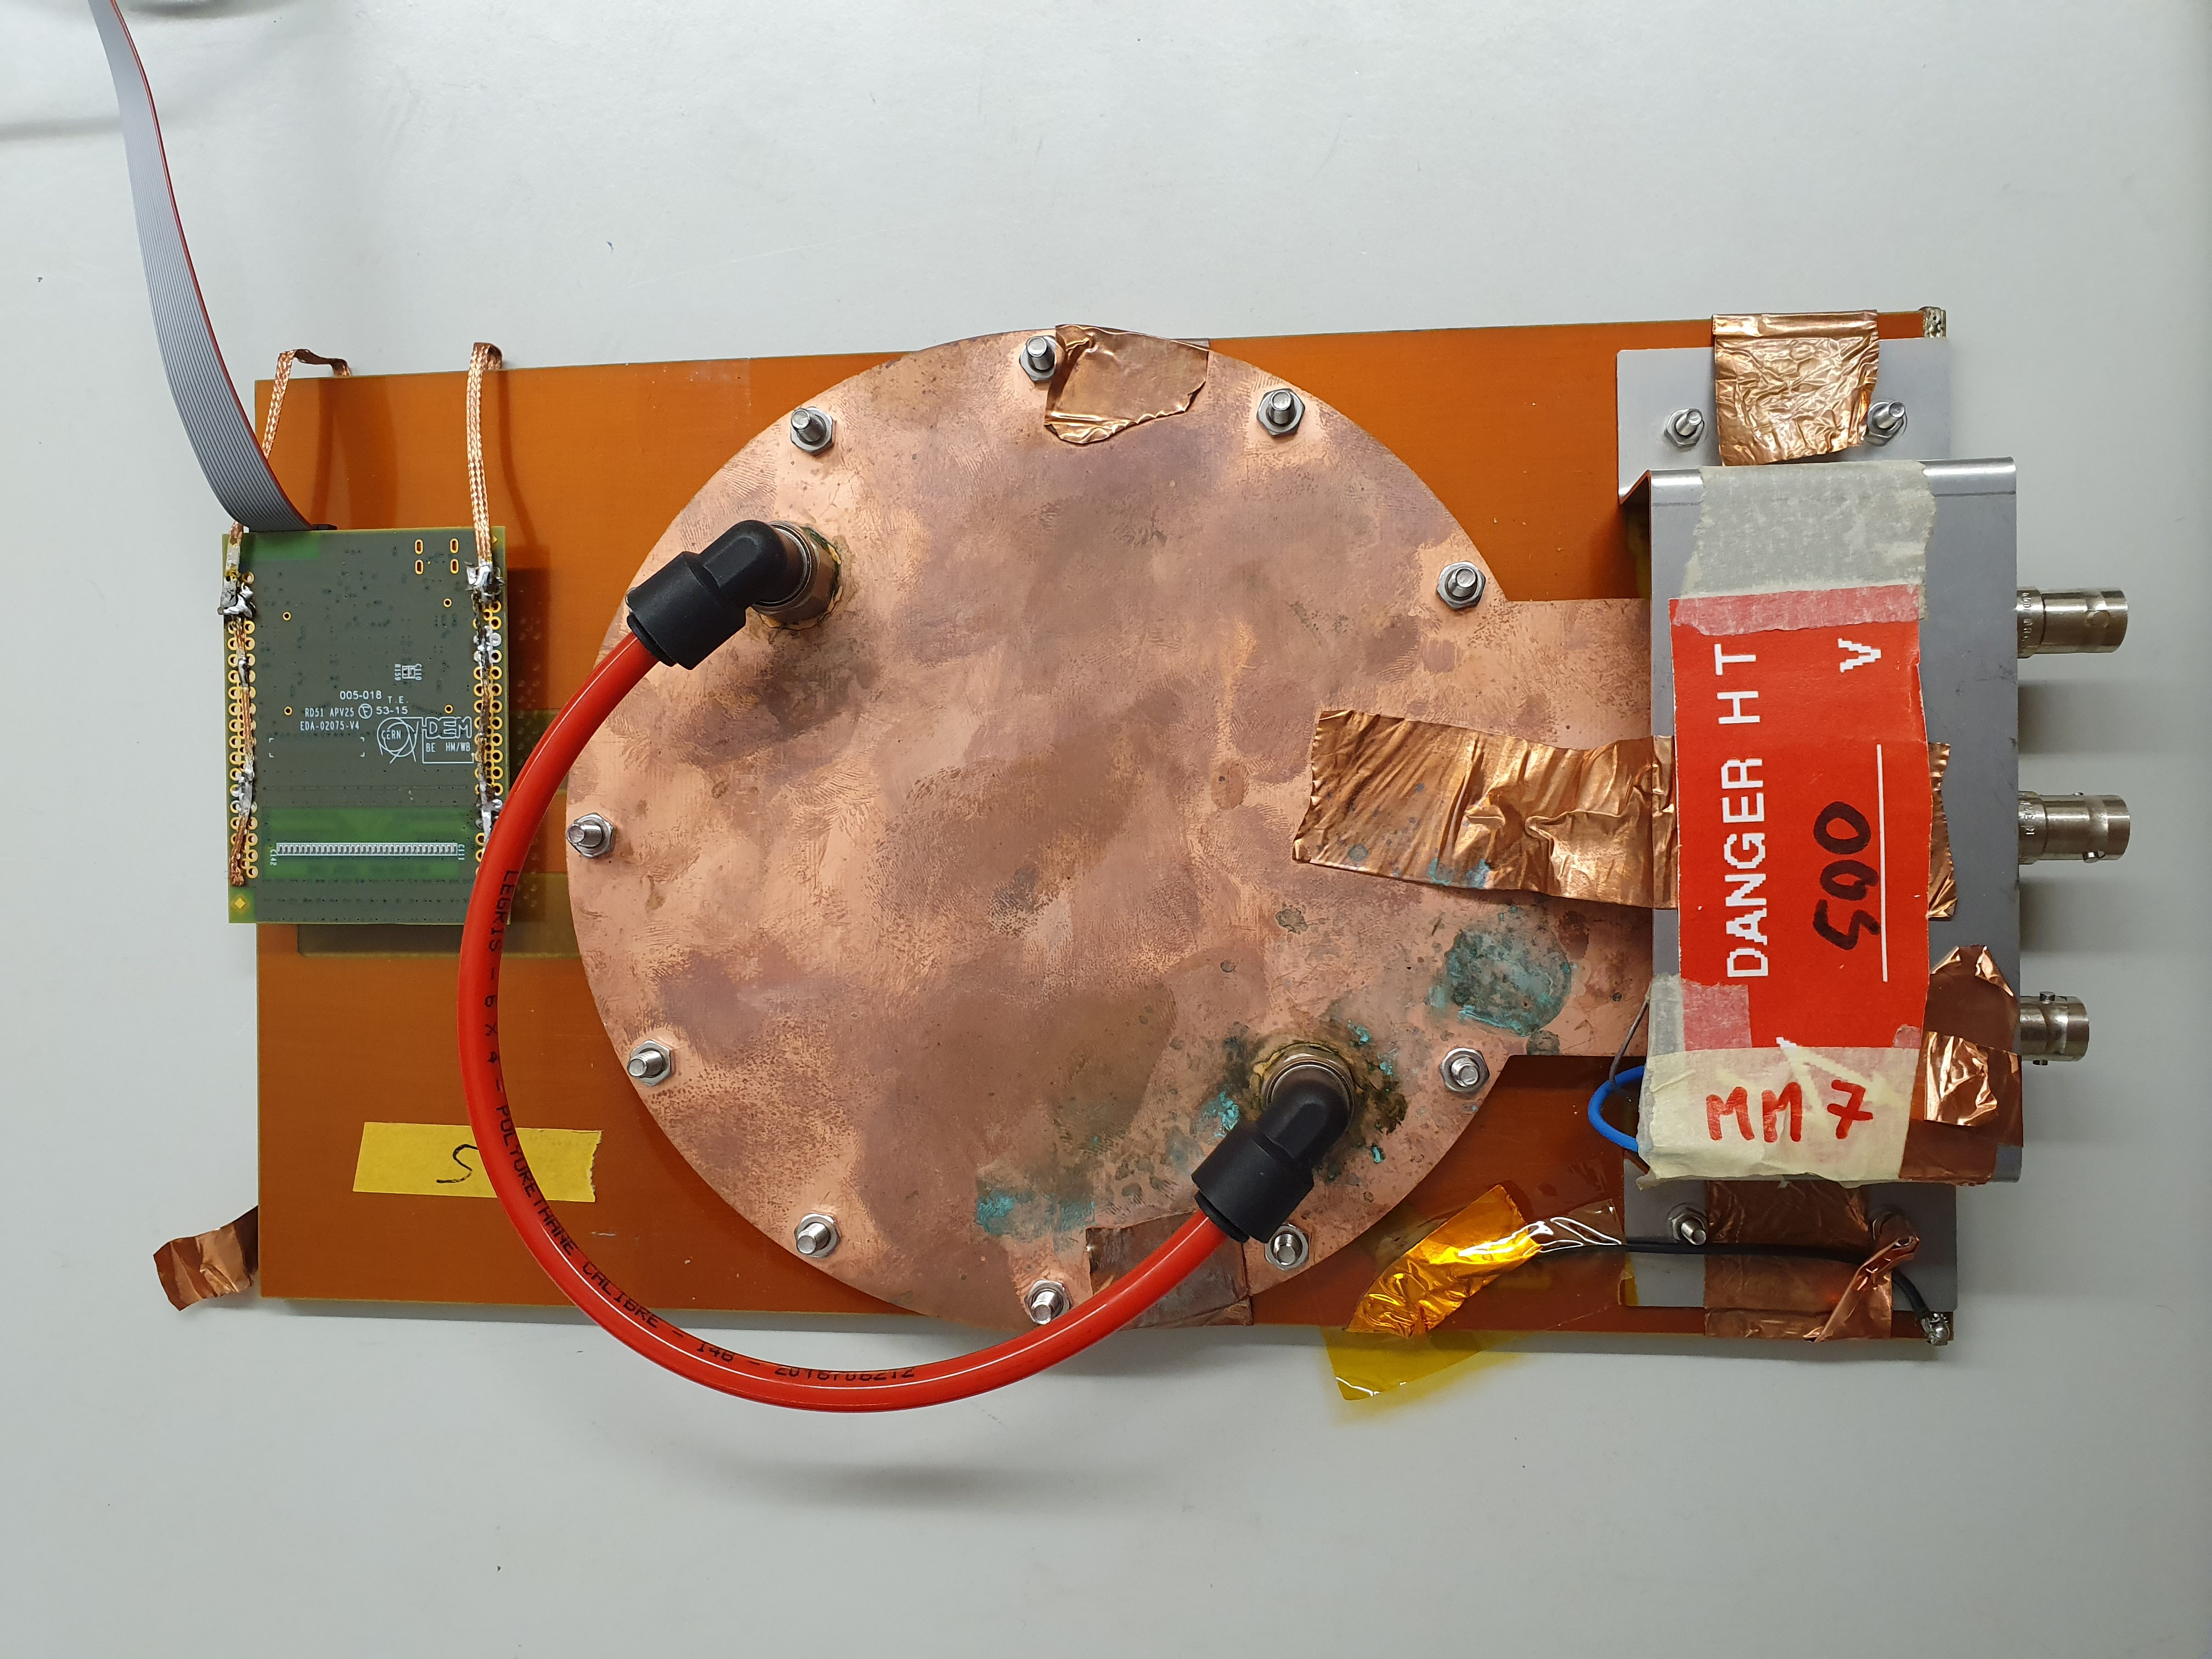
\includegraphics[width=\textwidth]{\pdirtwo/mm-photo-old.jpg}
  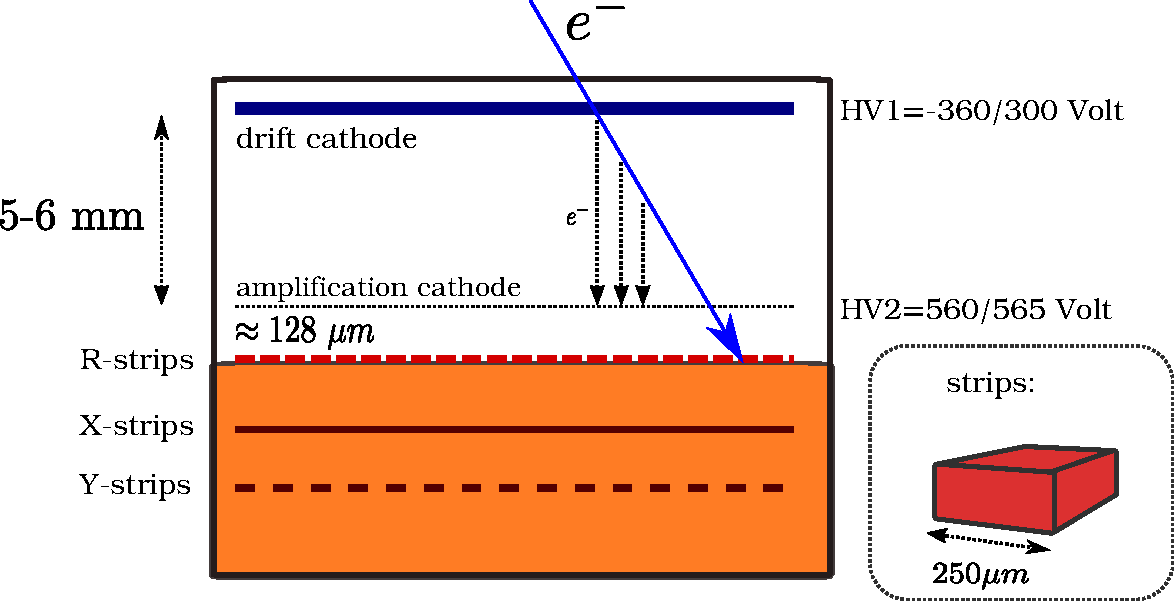
\includegraphics[width=\textwidth]{\pdirtwo/mm-principle.pdf}
\caption[Micromegas sketch]{Working principle and sketch of the Micromegas detector used in the NA64 experiment.}
\label{fig:mm-sketch}
\end{figure}

In the NA64 case, a negative voltage of 300-360 \si{\volt} (depending on the variable drift height) is applied to the drift plate. The mesh is connected to the ground while the resistive strips are kept at a positive voltage ranging from 560 and 565 \si{\volt} (due to some minor differences between MM). The resistive strips (R-strips) have a resistance of 1 \si{\mega\ohm} and are placed parallel to the X-strips. The Y-strips are placed after the R-strips and perpendicular to them. All set of strips have a pitch of 250 $\mum$, the width on the other hand is 200 $\mum$ for the R and X strips and 50 $\mum$ for the Y-strips.

Another important feature of this module is the genetic multiplexing of the strips: they are grouped in sets of five strips connected to a single channel. The results of this scheme are the reduction of the total number of channels needed for a complete readout of a module: the 640 strips of each micromegas (320 strips per plane) can be read by a single APV25 readout chip (see Sec.\ref{ch2:sec:daq}). The trivial disadvantage of multiplexing is a possible redundancy of the hit position of the incoming particle, which becomes more relevant as the occupancy of single event increases. To minimize this effect, one has to choose the mapping to maximize the separation between strips connected to the same channel, to make sure that no redundancy takes place. This technique was originally proposed in \cite{Procureur:2013yea}, and consist in distinguishing the original physical channel from the one created as an artifact by the multiplexing mapping by selecting as candidate clusters only the one where several (starting from a minimum of two) neighboring strips shows a signal over the threshold. An example of a single electron passing through a plane with different degrees of multiplexing can be seen in Fig.\ref{fig:multiplexing-example}. Producing the optimal mapping for the multiplexing where the redundancy is minimal is not a trivial task. Following \cite{Procureur:2013yea}, one can produce an optimal mapping if the number of channels to map is a prime number. If we consider a detector with $n$ strips that are to be read by a number $p$ of channels, we construct $(p-1)/2$ sublists containing the channel numbers $p$ according to the formula:

\begin{equation}
\label{eq:mm-multiplexing-mapping}
1 + [(i \times s) mod p]
\end{equation}

where $s$ is the number of the sublist and $i$ is ranging from 0 to $p-1$. In a more general case, Eq.\ref{eq:mm-multiplexing-mapping} can be used when the number of channels is not a prime number. In the NA64 case for example, where per plane we have a multiplexing factor of 5, and $n=320$, $p=64$ the sublists are still constructed following Eq.\ref{eq:mm-multiplexing-mapping}. Instead of using the number $s$ of the sublist a set of $(p-1)/2$ number $s_i$ is calculated to minimize the distance between neighboring strips mapped to the same channel $p$. The set $s_i$ is typically computed using numerical methods. The map for both planes of the 8 MM used is shown in Table \ref{tab:mm-map-original}. A new improved map is being prepared for the next generation of the NA64 experiment and will be discussed in chapter \ref{chapter4}.

\begin{figure}[bth!]
  \centering
  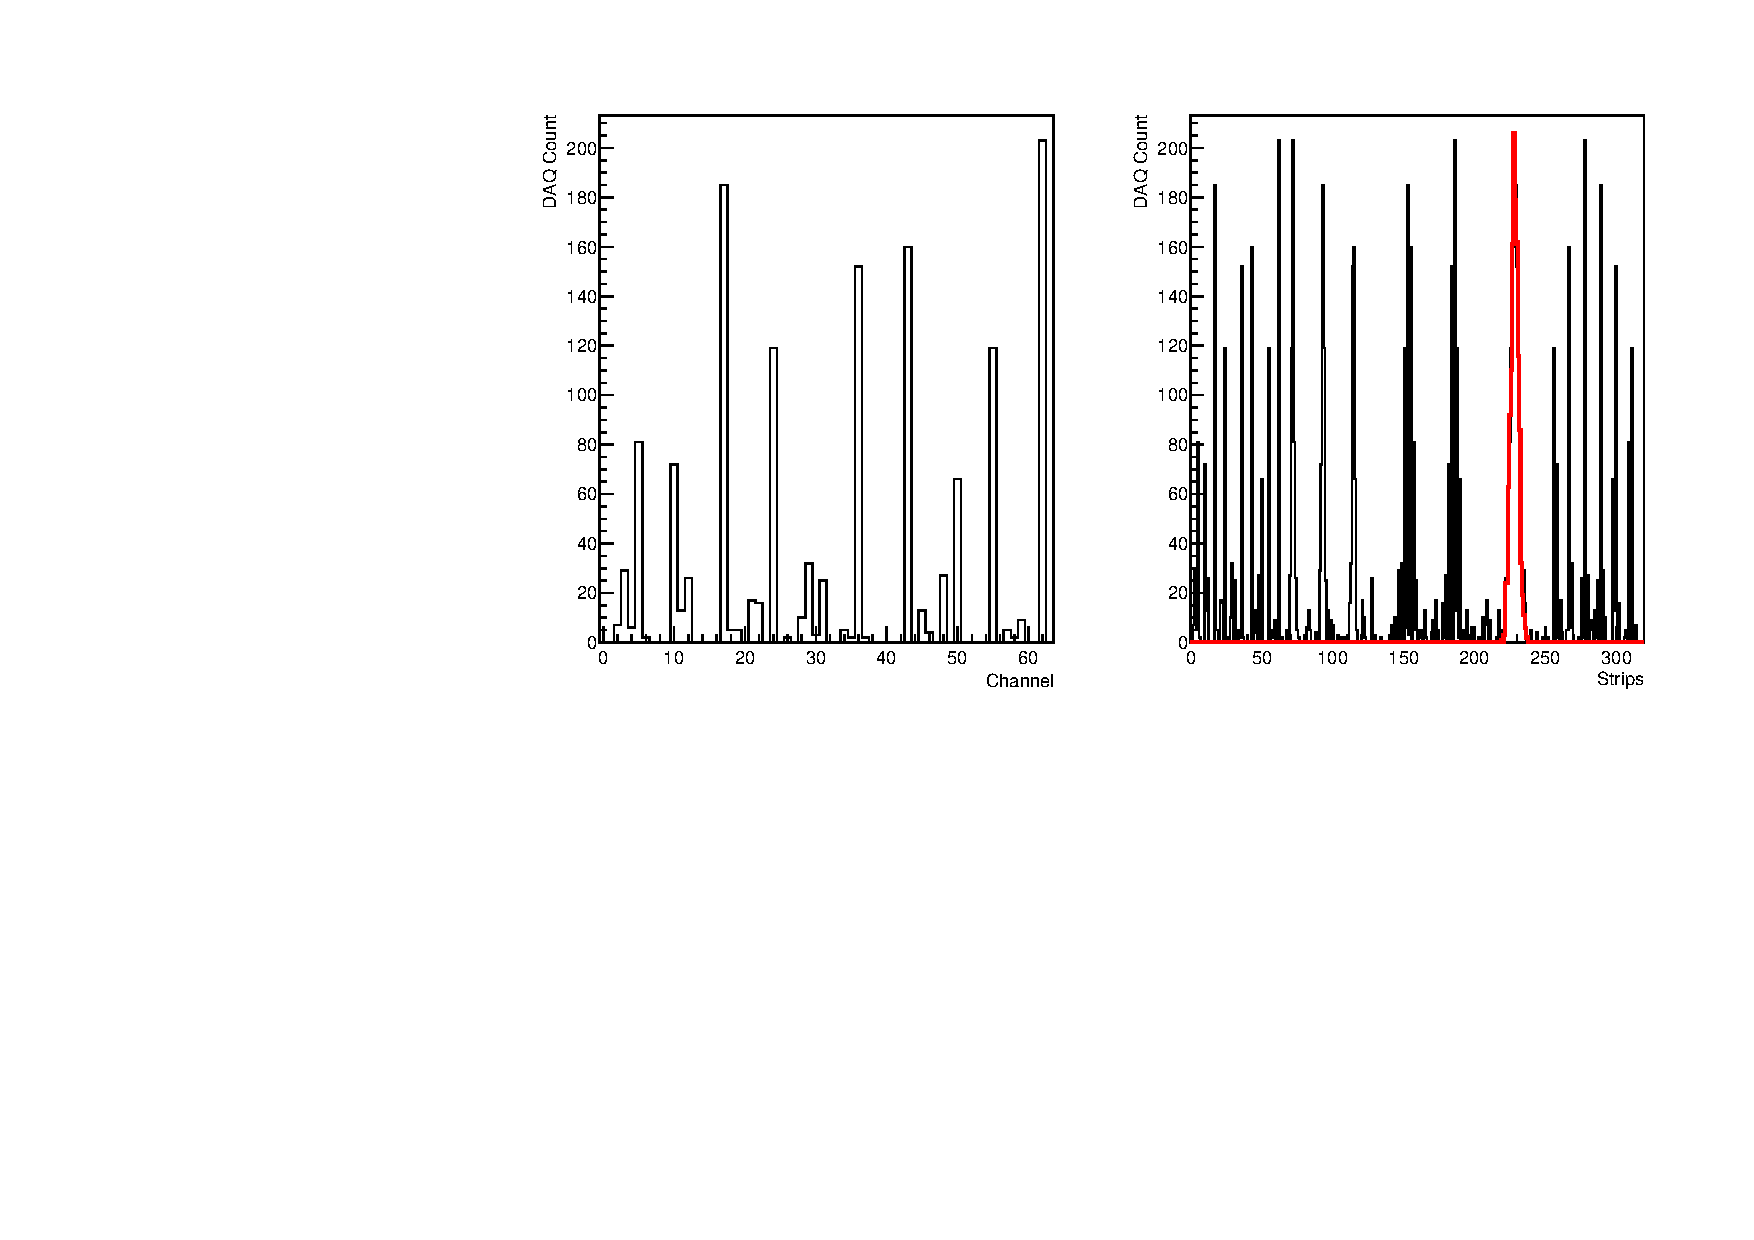
\includegraphics[width=\textwidth]{\pdirtwo/mm_output_example.pdf}
\caption[example of the readout of a multiplexing detector]{Left: example of the output in a Micromegas plane after the passage of a MIP. Right: same output transformed in the strips space using the multiplex map. The cluster selected by the reconstruction algorithm is shown in red.}
\label{fig:multiplexing-example}
\end{figure}

In NA64 the multiplexing feature was experimented for the first time in an high-intensity environment. The results however show that these trackers are capable of resisting the high flux of particles and allow a precise momentum reconstruction with a precision of $\simeq$1\% at 100 $\gev$ \cite{Banerjee:2017mdu}.

\subsubsection{GEM detectors}
\label{ch2:sec:gem}
The Gas Electron Multiplier (GEM) is a gaseous tracking detector based on a similar principle of the Micromegas. Their performance is similar for both hit resolution, radiation hardness, material budget, and total active area. The working principle is described in detail in \cite{gem,SAULI20162,ABBON2007455}.

GEM consists of a composite grid of two metal layers separated by a thin insulator (typically Kapton) etched with a regular matrix of open channels. The two metal layers on the opposite side of the grid are kept at a suitable potential difference to create a large field in the hole. Secondary electrons are created by the primary during its passage in the gas and are amplified by the electric field during their drift through the holes. Electrons produced in this multiplication region are then collected by electrodes to measure the impact position of the original particle. To increase the signal GEM can stack multiple plates in series to increase the charge multiplication.

In NA64, the GEMs are produced stacking three consecutive foils to amplify the original signal of the secondary electrons. This allows the detector to reduce the voltage difference between foils to a minimum to ensure a low amount of discharge and allow them to operate efficiently ($\sim$99\% MIP efficiency) in the high intensity of the H4 beamline. Each foil has an area of 100$\times$100 $\mms$ with a hole pitch of 140 $\mum$. The readout consists of a two-layer strip anode with 256 strips per plane and a pitch of 400 $\mum$. Like the MM, the signal from each strip is processed by 128 channels APV chips, for a total of 4 chips to read out all strips for both XY plane.
One of the main differences between the two types of detectors is that GEM trackers are not multiplexed, meaning that every single strip is readout by a single electronic channel. For the momentum reconstruction, where only one primary particle hits the tracker in a single event, both MM and GEM detector performs similarly due to the multiplex map properties. When more then one particle hits the trackers, a multiplexed detector can create some redundancy that potentially limit the efficiency and bias the exact hit position. For this reason, GEM detector was placed inside the decay volume during the 2018 visible mode run to maximize the efficiency for signal events, where a $\ee$ is present inside the decay volume.

\subsection{The data Acquisition system (DAQ)}
\label{ch2:sec:daq}

The DAQ used for NA64 is a downscaled version of the COMPASS DAQ system \cite{Bodlak_2013,COMPASS-daq}. The detector's frontends are connected to the readout modules that with a processing speed up to 160 MB/s organize the digital information received by the frontends electronic into a preliminary event-like structure (sub-event building) (see Fig.\ref{fig:daq}). Triggers and control information are passed to these modules via the Trigger Control System (TCS), which work synchronously with the SPS duty cycle and creates the header and distributes it containing the spill number, the event number, and the trigger type later used by the event builder PC. Two types of readout modules are used in NA64: the CATCH (Compass Accumulate Transfer and Cache Hardware), a general readout module that supports a wide range of frontend electronics, and the GeSiCa (Gem Silicon Control and Acquisition), which is optimized for the readout of the APV25 frontend chip that is used by both Micromegas and GEM detectors.

The APV25 is an ASIC that combines analog signals with a digital control \cite{Bodlak_2013} originally developed for the readout of the CMS silicon trackers \cite{article,inproceedings,apv-useguide}. Each of the 128 channels of the chip are made by a 60 $\nas$ CR-CR shaping amplifier and a 192 samples deep analog pipelines. The amplifier integrates the current pulse from the input and output of a well-defined voltage pulse. A 192 samples deep analog pipeline is used to store the amplifier output to wait for the external trigger decision. This pipeline is made of switched-capacitor elements. 160 of the 192 memory cells are organized in a ring buffer with a write and trigger pointer. The distance between the two defines the trigger latency which is a configurable parameter. When one of the pipeline columns is flagged for readout, it is copied into one of the remaining 32 memory elements, organized like a FIFO\footnote{\textbf{F}irst \textbf{I}n \textbf{F}irst \textbf{O}ut is a form of data buffer that conserves the order of the incoming data.}. The data are stored here until are sent out by the multiplexer. Then, the data is sent to an ADC\footnote{\textbf{A}nalog to \textbf{D}igital \textbf{C}onverter} modules (which can accommodate up to 4 APV chip) that digitizes the pulse before sending it to the GeSiCa. The ADC has two possible modes of operation, the latch-all mode, and the sparse mode. When using the latch-all mode, the signal amplitudes of all channels is sampled three times with a clock cycle of 25 $\nas$ and transmitted to the GeSiCa. In this mode the trigger rate cannot be higher than $\sim$1 \si{\kilo\hertz} due to the large amount of data received by the APV25. To reach higher trigger rates, the sparse mode is used instead. When in sparse mode, only channels with amplitudes above a certain threshold are sent to the GeSica by the ADC module. This allows us to increase the manageable trigger rate to $\sim$10 \si{\kilo\hertz}. In NA64, the latch-all mode is used to record the data coming by the APV25 connected to the trackers but in absence of the beam. This procedure is repeated every $\sim$10-15 run approximately to record the pedestal of each channel. The pedestal recorded are then used to set the threshold (2$\sigma$ for MM and 3$\sigma$ for GEMs) for the sparse mode, which is used during data taking to maximize the trigger rate.

\begin{figure}[tbh!]
\centering
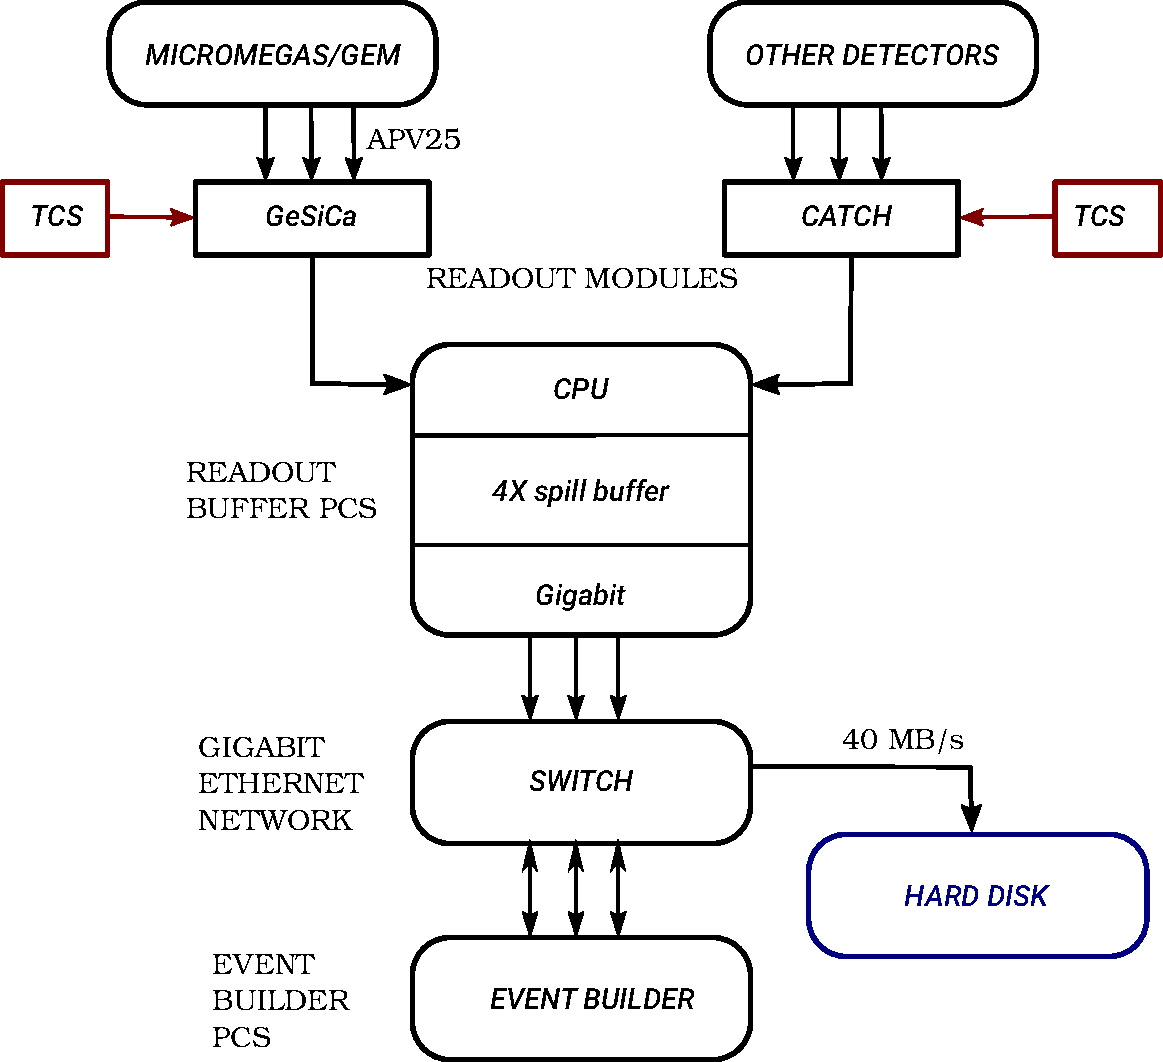
\includegraphics[width=\textwidth]{\pdirtwo/daq.pdf}
\caption{Scheme for the NA64 DAQ}
\label{fig:daq}
\end{figure}

During the calibration procedure, the three samples received by each channel of the APV25 are also used to set the latency of the trigger. The latency of the trigger is optimal when it covers precisely the rising edge of the pulse received by each channel of the APV25. If we define a$_0$, a$_1$ and a$_2$ as the three samples recorded in consecutive order by a single APV25 pipeline, the latency is to be set such that the second sample a$_1$ is larger than the other two amplitudes. This can be best summarized in the so-called "banana plot" of Fig.\ref{fig:banana-plot}, which is a heat map plotting the frequency of events with certain pulse structure. The sampling of the pulse shape also provides additional information about the time of arrival of the primary electron. By reconstructing the pulse shape rise time one can improve the time estimate by the usual 25 $\nas$ (limited by the clock frequency of the APV) down to $\sim$15 $\nas$ \cite{Banerjee:2017mdu}. To achieve this, the pulse is described by the following function:

\begin{equation}
\label{eq:apv-pulse}
r(t) = \frac{r_0}{(1 + \exp{\frac{t-t_0}{\tau}})}
\end{equation}

Where the parameters $r_0$, $t_0$ and $\tau$ are fitted using the same data measured at different values of the latency. The time of arrival is then extracted by reversing the function and solving it as a function of the ratio between pulses:

\begin{equation}
\label{eq:2}
t(r) = t_0 + \tau \times \ln{\frac{r_0}{r} - 1}
\end{equation}

A complete description of the method that takes into account the errors of the ratio and the parameters can be found in \cite{dbanerjee-thesis}.

\begin{figure}[!bth]
  \centering
  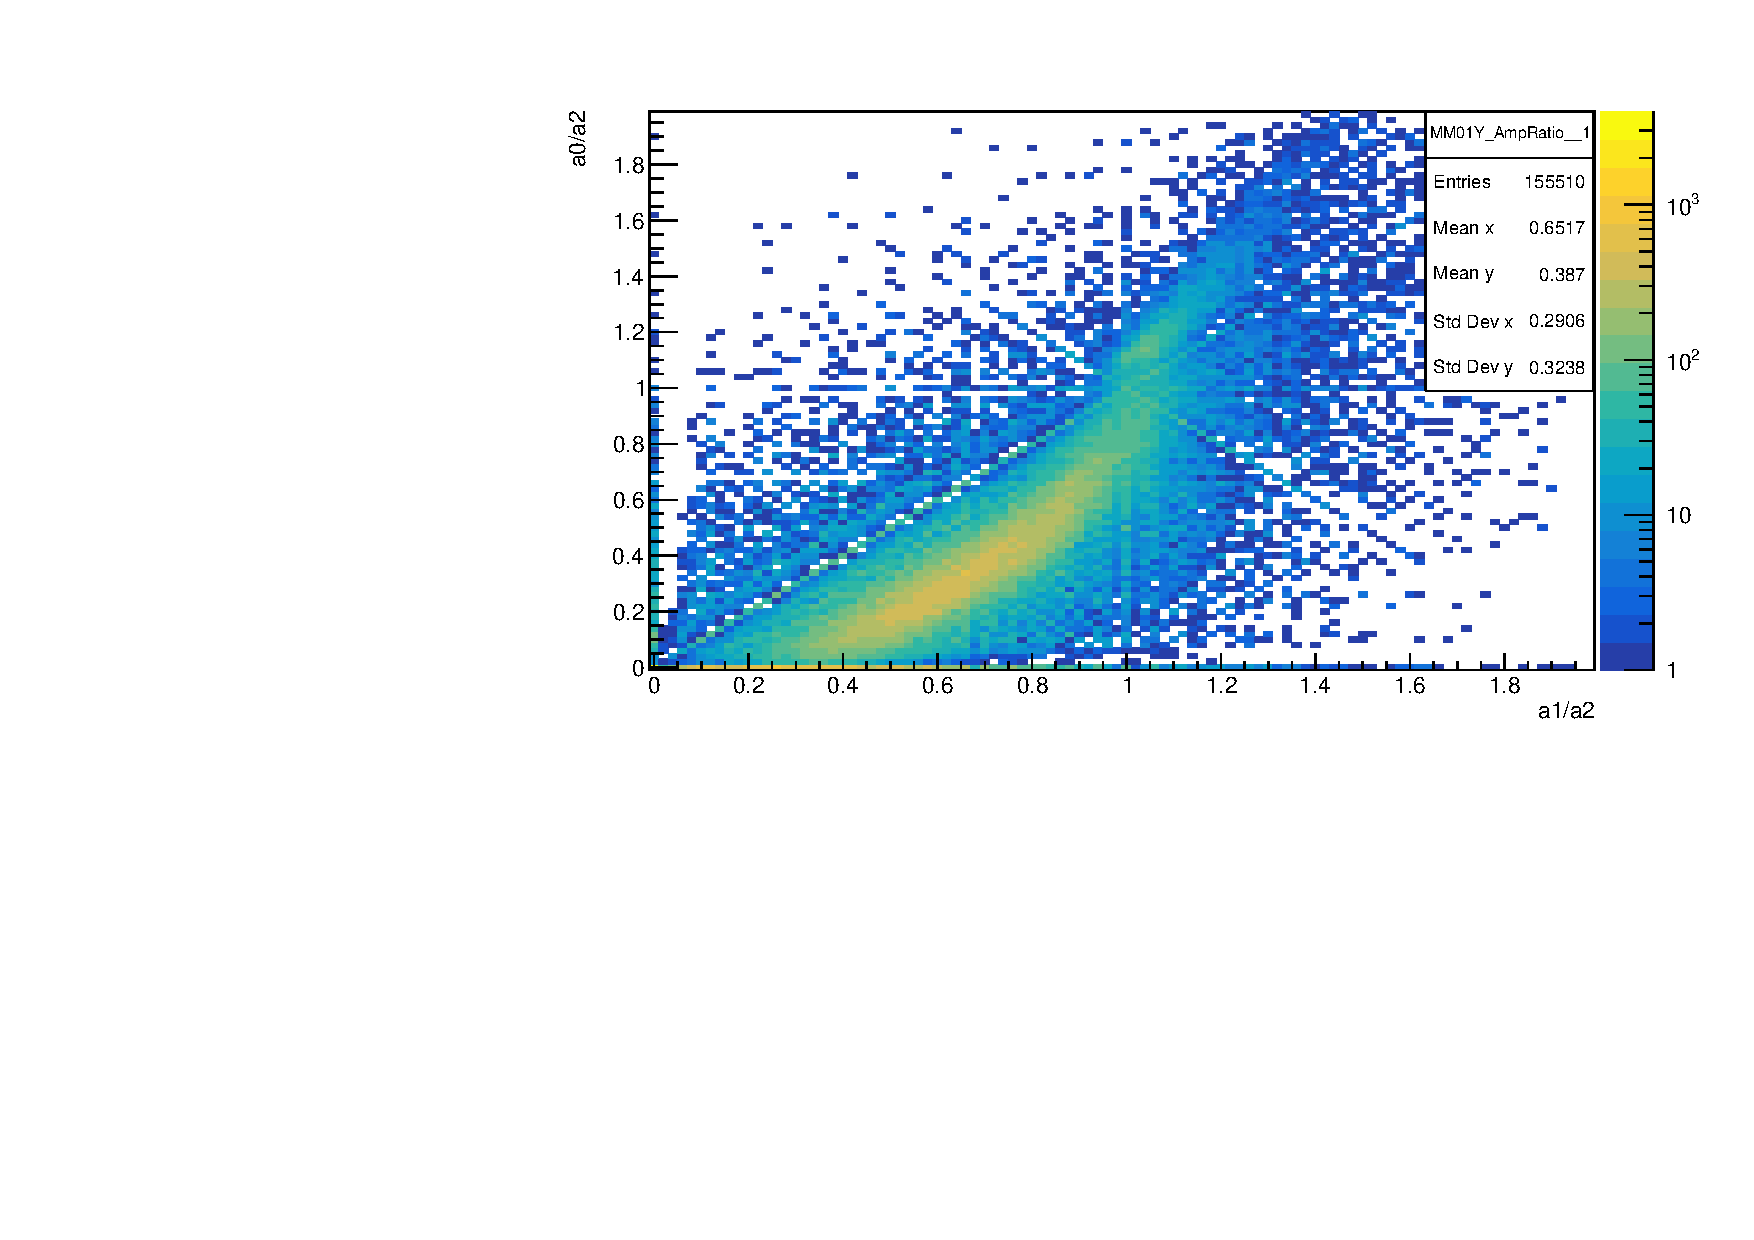
\includegraphics[width=\textwidth]{\pdirtwo/MM1Y_bp.pdf}
\caption[APV25 banana plot]{Ratio between the first two vs the last two amplitudes sampled in an APV25 chip after the proper latency is set for the chip. The typical "banana" shape of this plot is the sign that the pulse is sampled during its rising edge.}
\label{fig:banana-plot}
\end{figure}

After passing through the ADC, the data is sent to GeSica using a high-speed optical cable. The Gesica can accommodate up to 4 ADC (for a total of 16 APV chips) and has the purpose of multiplexing the incoming data stream, merging the header information from the TCS\footnote{Trigger Control System} with the corresponding data coming from the APV, and finally putting the event data block into the S-link format. Finally, the information are transferred to a high-performance readout buffer PCs (ROB) via the S-link protocol\footnote{The S-link is a protocol developed at CERN for fast point to point connections, typically between front-end electronics and the readout electronics \cite{s-link}.}. In the NA64 case, to accommodate the many GeSica and CATCH modules used, and S-link multiplexer is used to combine multiple modules before sending the data to the ROB. As seen in Fig.\ref{fig:daq}, the Readout buffer PCs receive the information from the multiplexer and stores them in four different spill buffer\footnote{A spill is a 512 MB SDRAM module which can store the data of at least one spill \cite{COMPASS-daq}}. A Gigabit Ethernet\footnote{Gigabit Ethernet is a standard developed by the Institute of Electrical and Electronics Engineers(IEEE) and Local Area Networks (LANs).} switch connects the ROB with the event builders PC. Here the data of every single event is merged into a single event data block using the event identifier provided by the TCS receiver. After this process, the event is ready to be recorded to the long term storage, in this case of 5 TB SATA Hard Disk with a speed of 40 MB/s. Thanks to this design the DAQ takes advantage of the beam structure of the H4, characterized by a high intensity for 4.8 \si{\second} where the spill buffers are filled by the information coming from the readout modules followed by a long recovery time of $\sim$20 \si{\second} that are used for the event building and to write all the information to the tape.

%%% Local Variables:
%%% mode: latex
%%% TeX-master: "../PhDthesis"
%%% End:
